\documentclass[handout]{beamer}

\usepackage{parskip, subcaption}

\title
  {A life-cycle based environmental and economic assessment tool for production systems}

\author
  {Roar Nind Steffensen (s144107)}

\date
{July 2018}

\institute
  {Technical University of Denmark}

\begin{document}

\maketitle

\begin{frame}{Introduction}
Contents
\begin{itemize}
    \item Life Cycle Assessment - Overview
    \item Requirements
    \item Program Overview
    \item Testing
    \item Decisions
    \item Demo
    \item Additional Topics
\end{itemize}
\end{frame}

\begin{frame}
\begin{center}
    \Large
    Life Cycle Assessment - Overview
\end{center}
\end{frame}

\begin{frame}{Life Cycle Assessment - Overview}
\begin{figure}
    \centering
    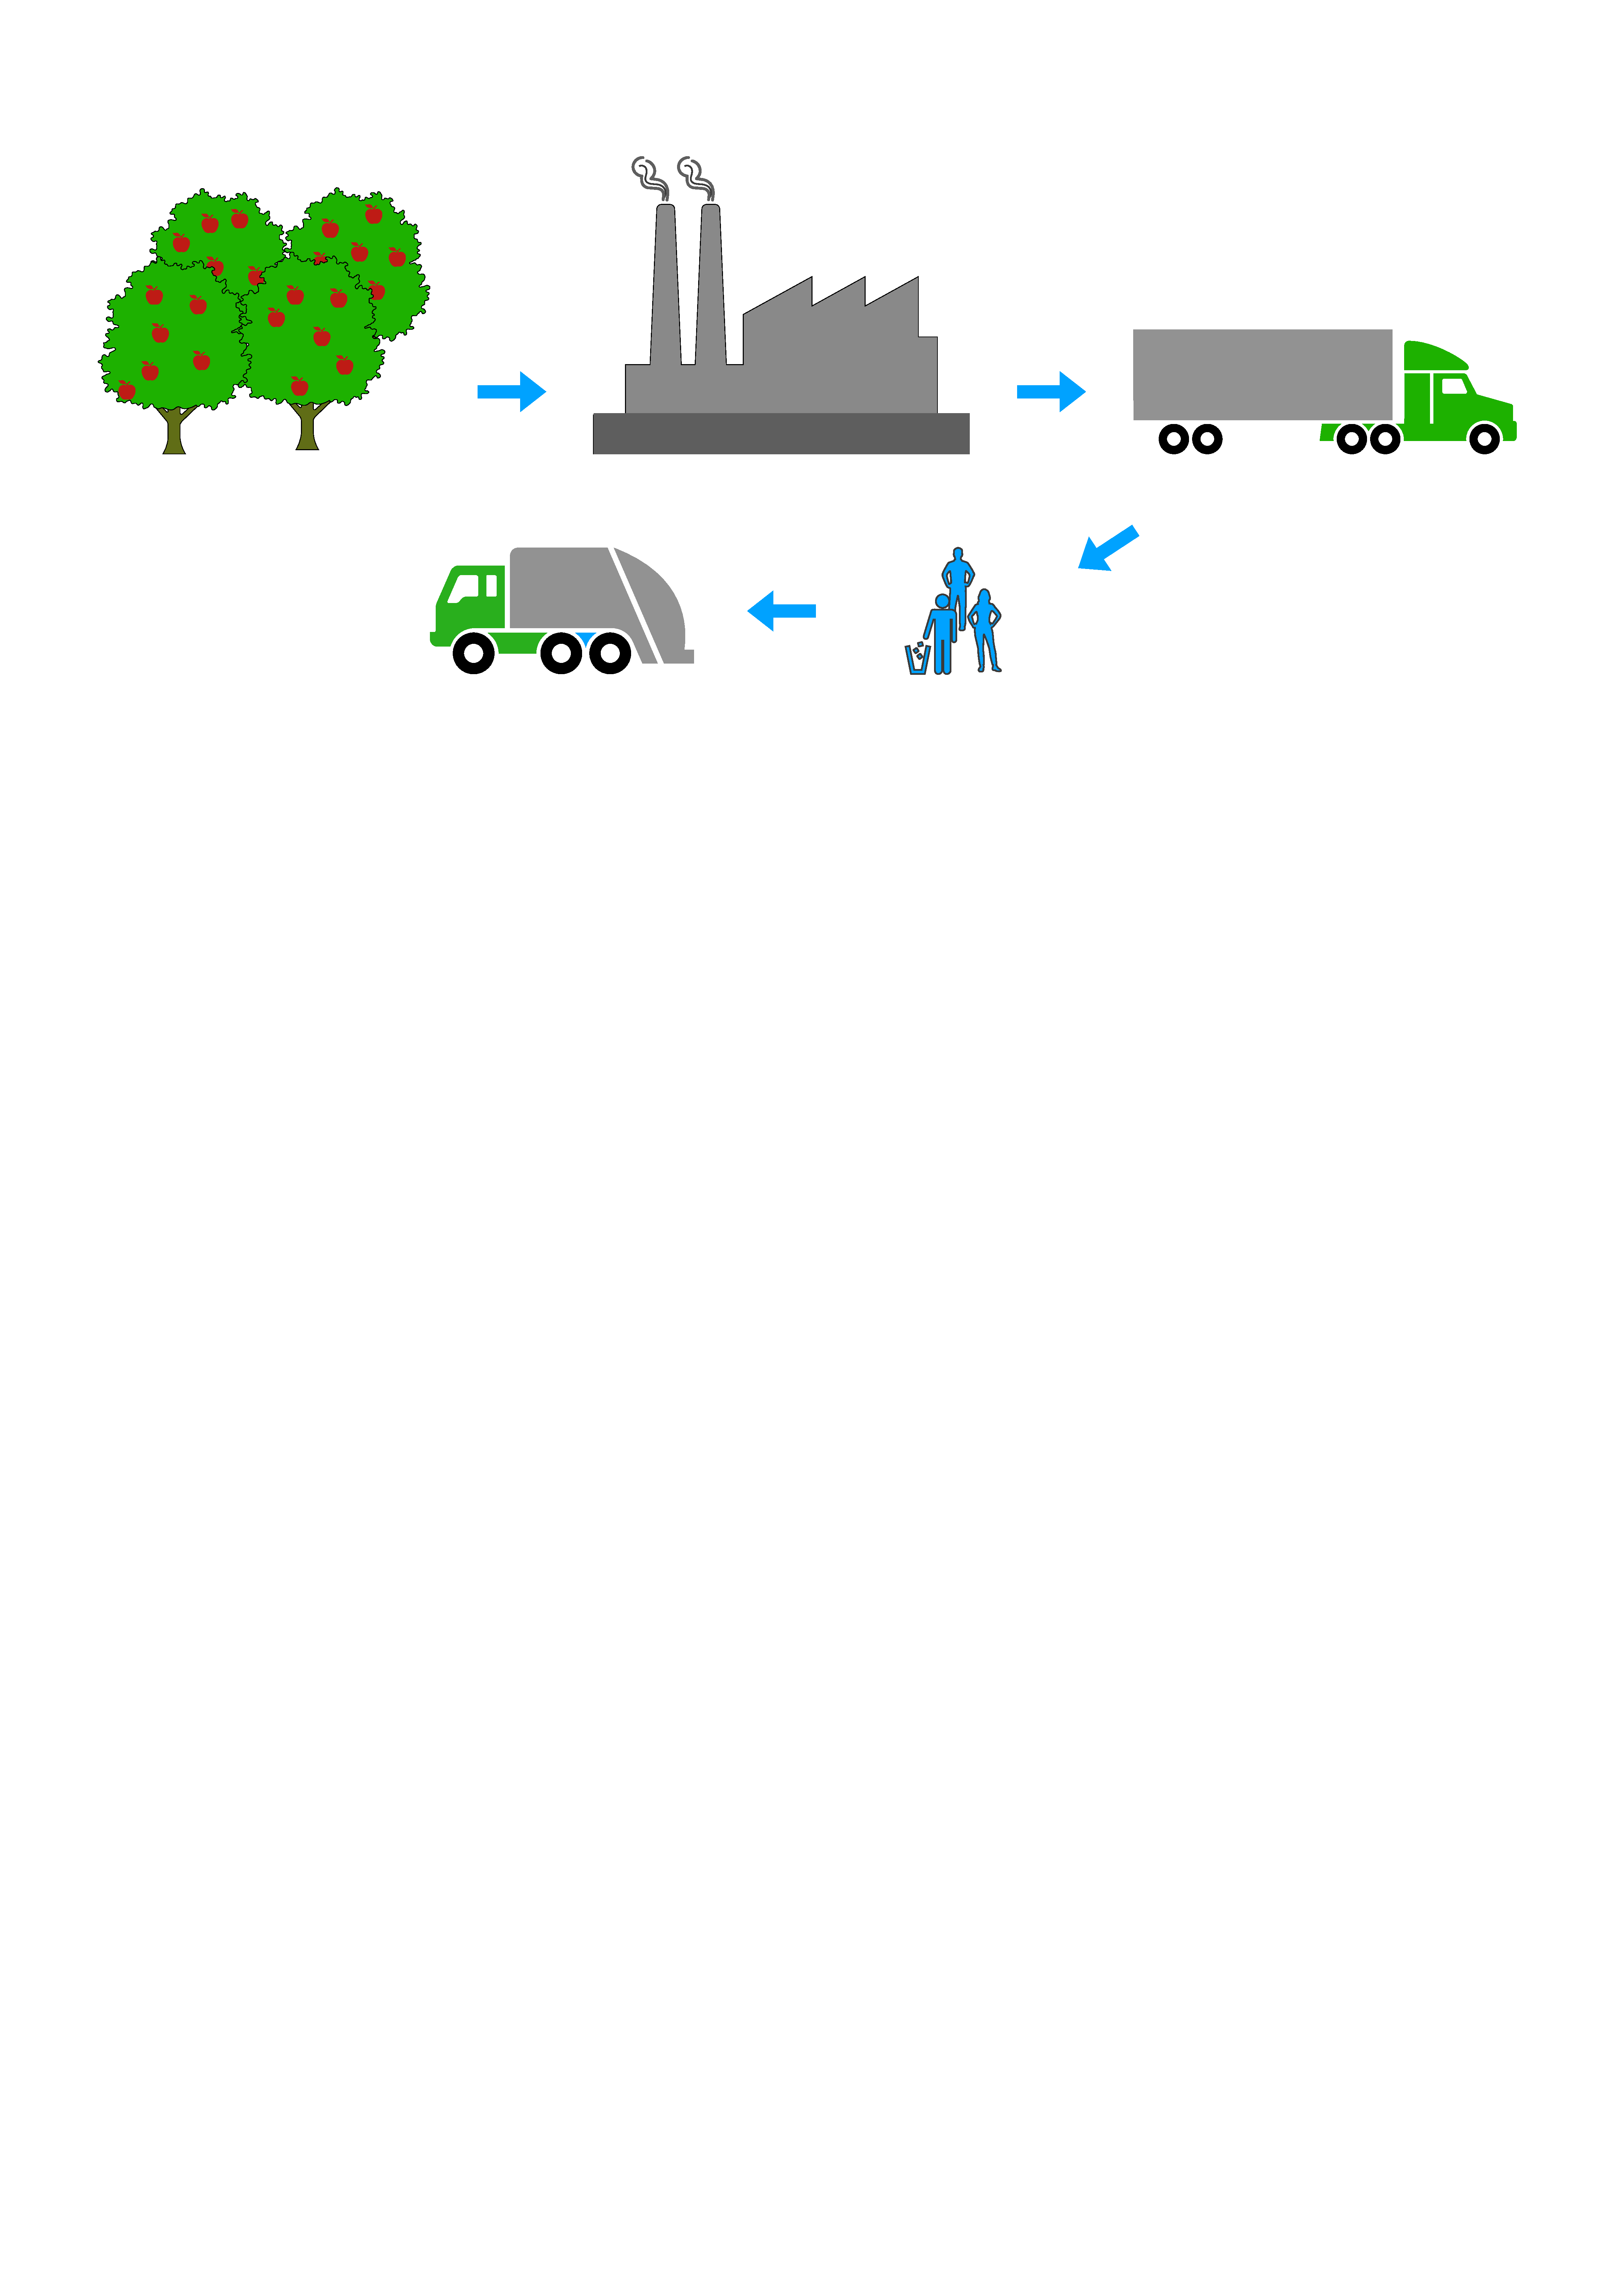
\includegraphics[width = 0.7\linewidth]{.figures/AppleJuiceExample.pdf}
    \caption{Apple juice production system example.}
\end{figure}
\end{frame}

\begin{frame}{Life Cycle Assessment - Overview}
Four phases of LCA:
\begin{enumerate}
    \item Goal and Scope
    \item Life Cycle Inventory (LCI)
    \item Life Cycle Impact Assessment (LCIA)
    \item Interpretation
\end{enumerate}
\end{frame}

\begin{frame}{Life Cycle Assessment - Overview}
\begin{figure}
    \centering
    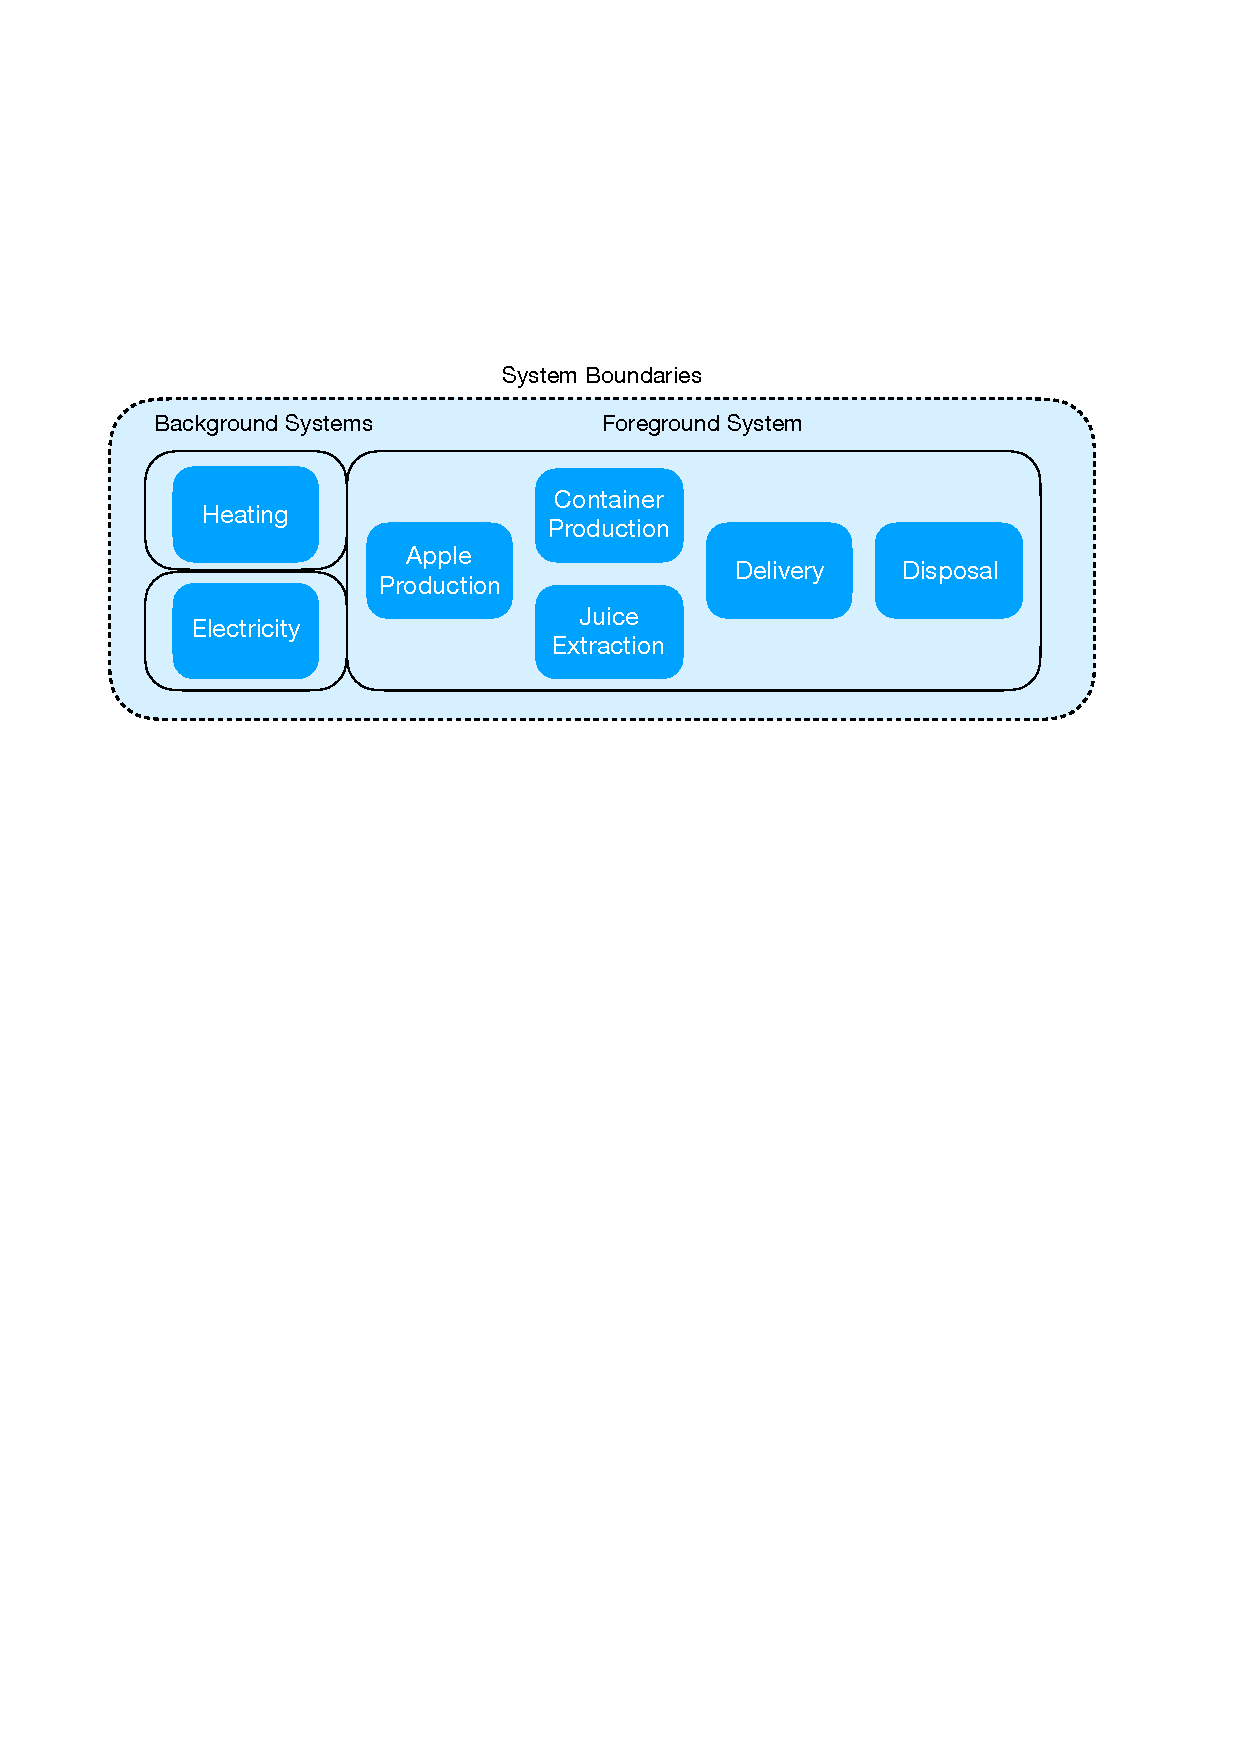
\includegraphics[width=1\linewidth]{.figures/InventoryComponents.pdf}
    \caption{LCI components for apple juice production}
\end{figure}
\end{frame}

\begin{frame}{Life Cycle Assessment - Overview}
From \textit{Life Cycle Assessment - Theory and Practice}:
\begin{center} \color{darkgray}
    \textit{"Calculate LCIA results per impact category:\\ 
    For each impact category separately, calculate the LCIA indicator results by multiplying the amount of each contributing (i.e. classified) elementary flow of the inventory with its characterisation factor. The results may be summed up per impact category, but summing up shall not be done across impact categories"}
\end{center}
\end{frame}

\newcommand{\red}[1]{{\color{red}#1}}
\begin{frame}{Life Cycle Assessment - Overview}
From \textit{Life Cycle Assessment - Theory and Practice}:
\begin{center} \color{darkgray}
    \textit{"Calculate LCIA results per impact category:\\ 
    For each impact category separately, calculate the LCIA indicator results by \red{multiplying} the amount of each contributing (i.e. classified) \red{elementary flow} of the inventory with its \red{characterisation factor}. The results may be \red{summed up per impact category}, but summing up shall not be done across impact categories"}
\end{center}
\end{frame}
\begin{frame}
\centering
\Large
Requirements
\end{frame}

\begin{frame}{Requirements}
    \begin{itemize}
        \item Get model information from user
        \item Convert user input to usable data
        \item Create \emph{dynamic} LCI model
        \item Calculate resulting impact
        \item Provide feedback of results
    \end{itemize}
\end{frame}







\begin{frame}{Traditional Aggregation}

\vfill
\begin{figure}
    \centering
    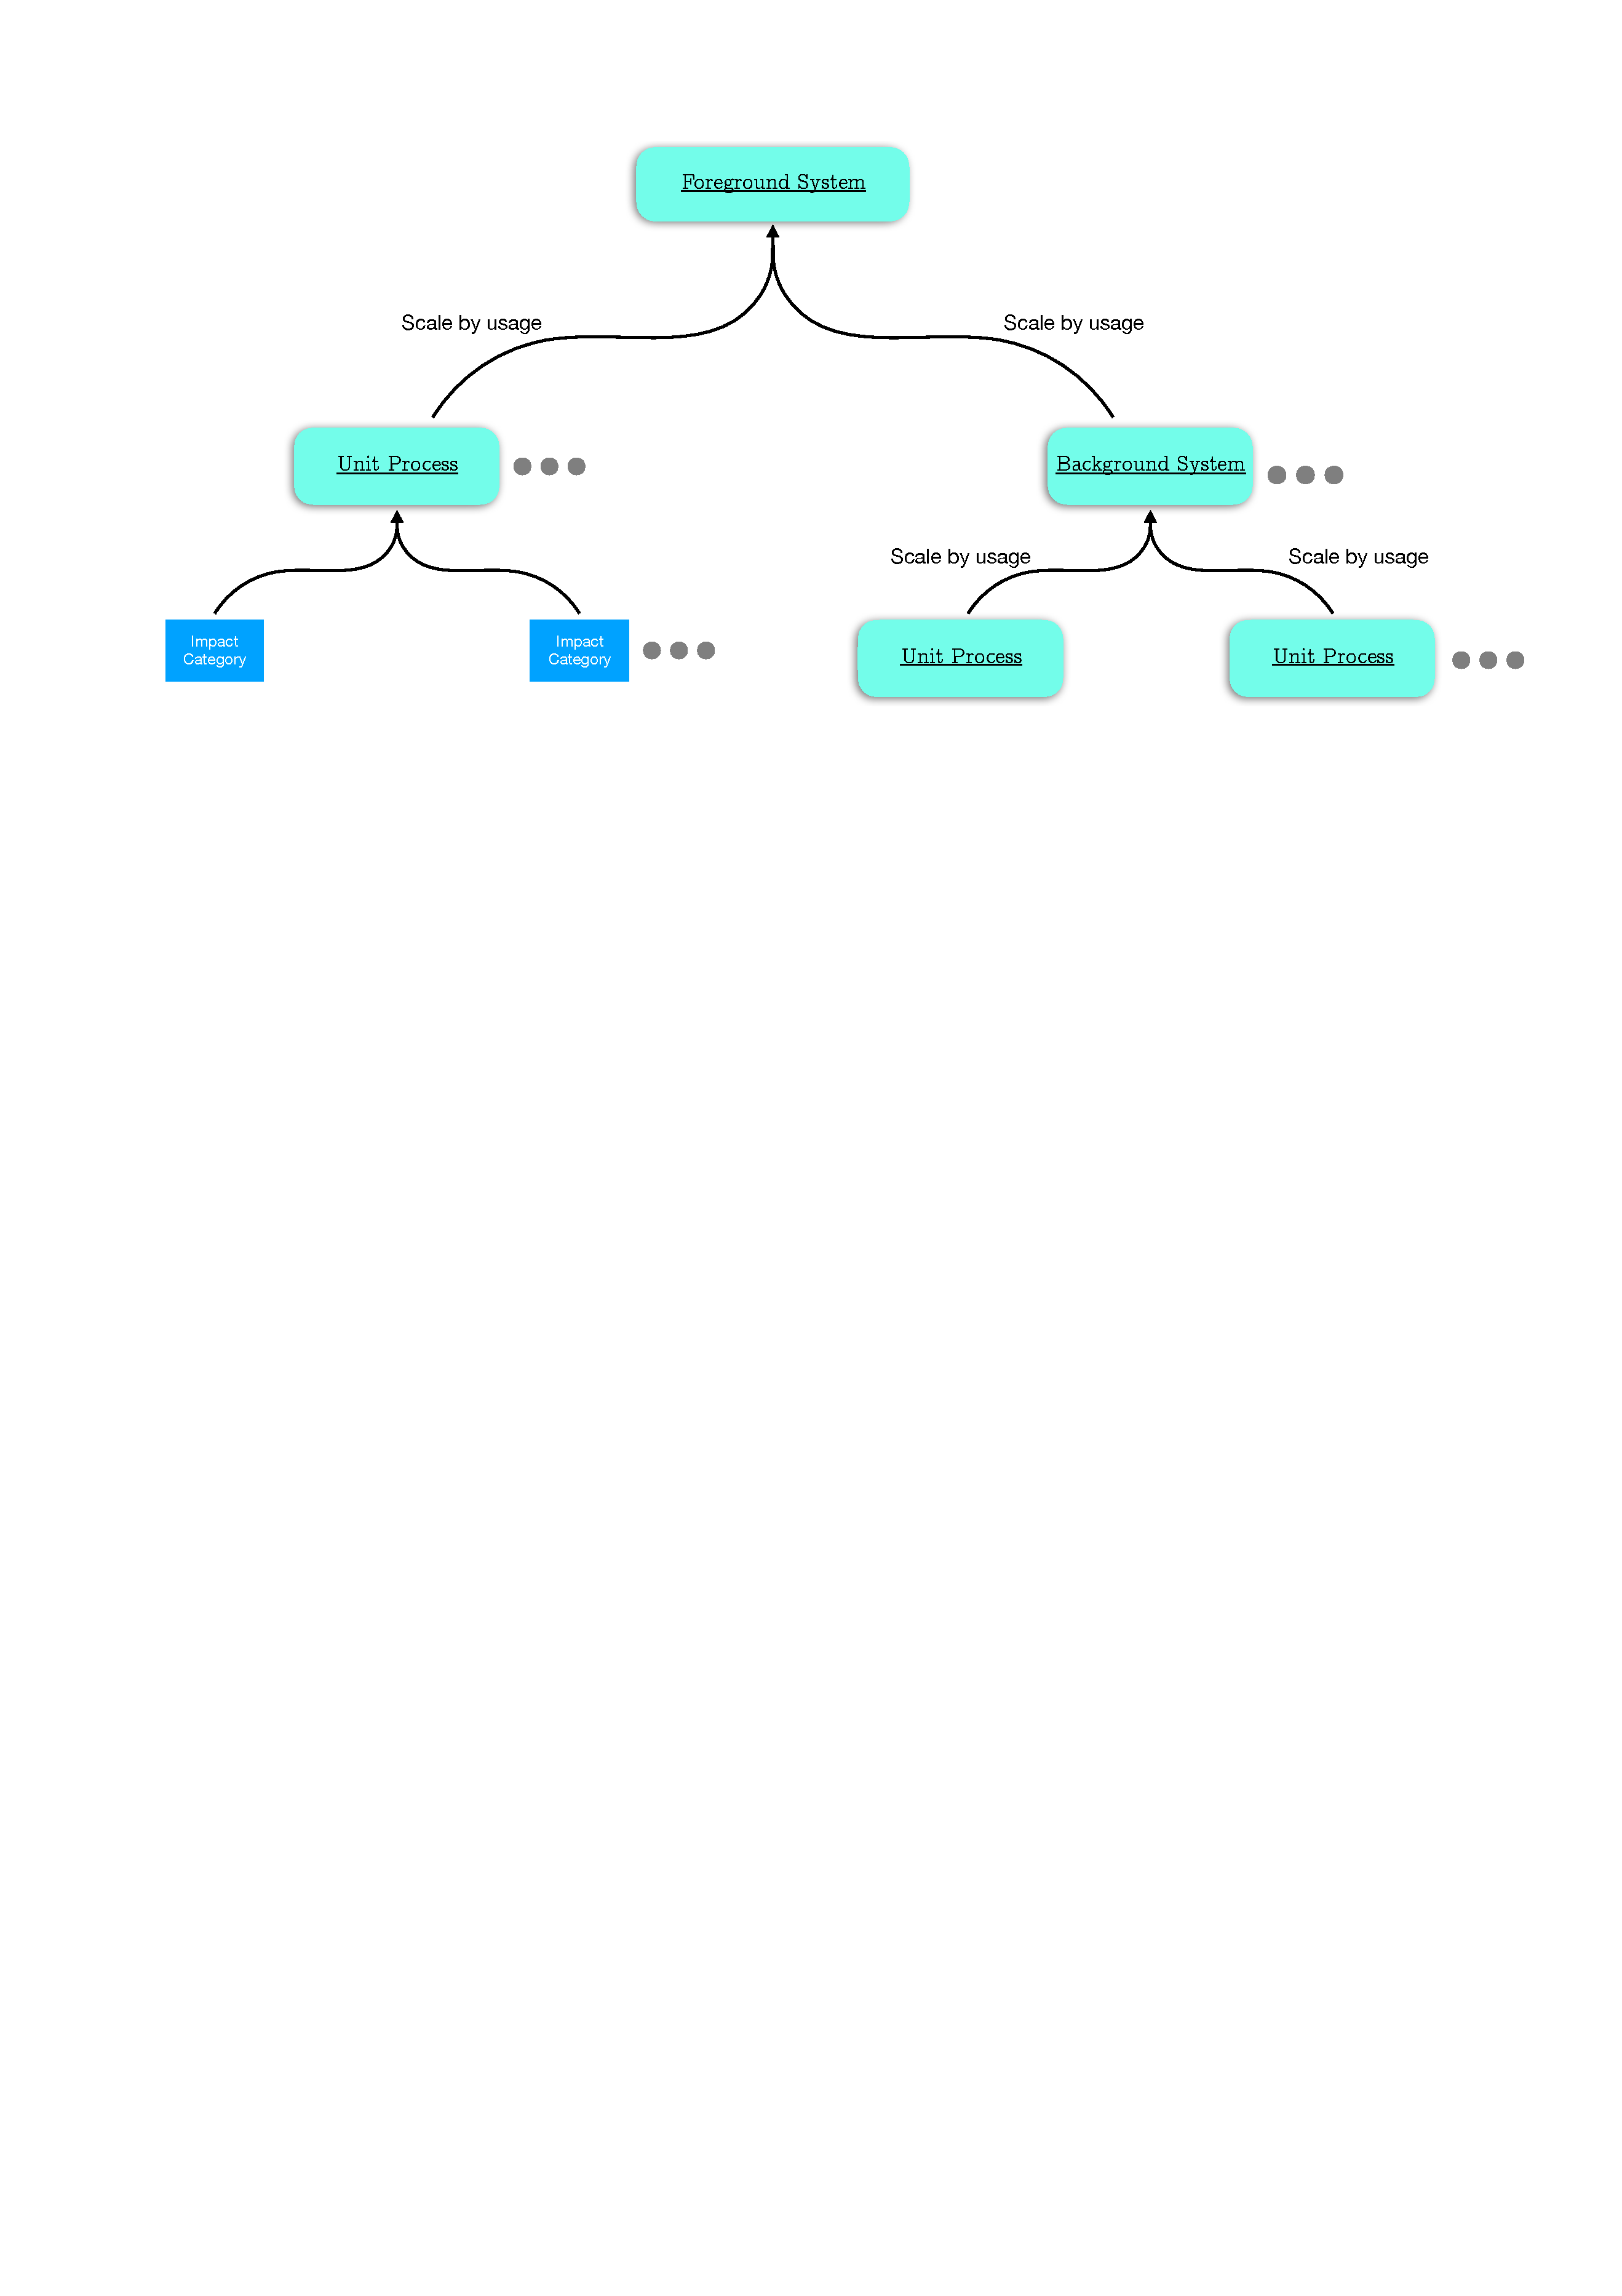
\includegraphics[page=1, width = \linewidth]{.figures/ImpactAggregationExtension.pdf}
\end{figure}

\end{frame}

\begin{frame}{Extended Aggregation}
\vfill
Extensions: Timestamped data values and dynamic properties.
\vfill
\begin{figure}
    \centering
    \includegraphics[page=2, width = \linewidth]{.figures/ImpactAggregationExtension.pdf}
\end{figure}

\end{frame}
\begin{frame}
\centering
\Large
Program Overview
\end{frame}

\begin{frame}{Objectives}

\begin{figure}
    \centering
    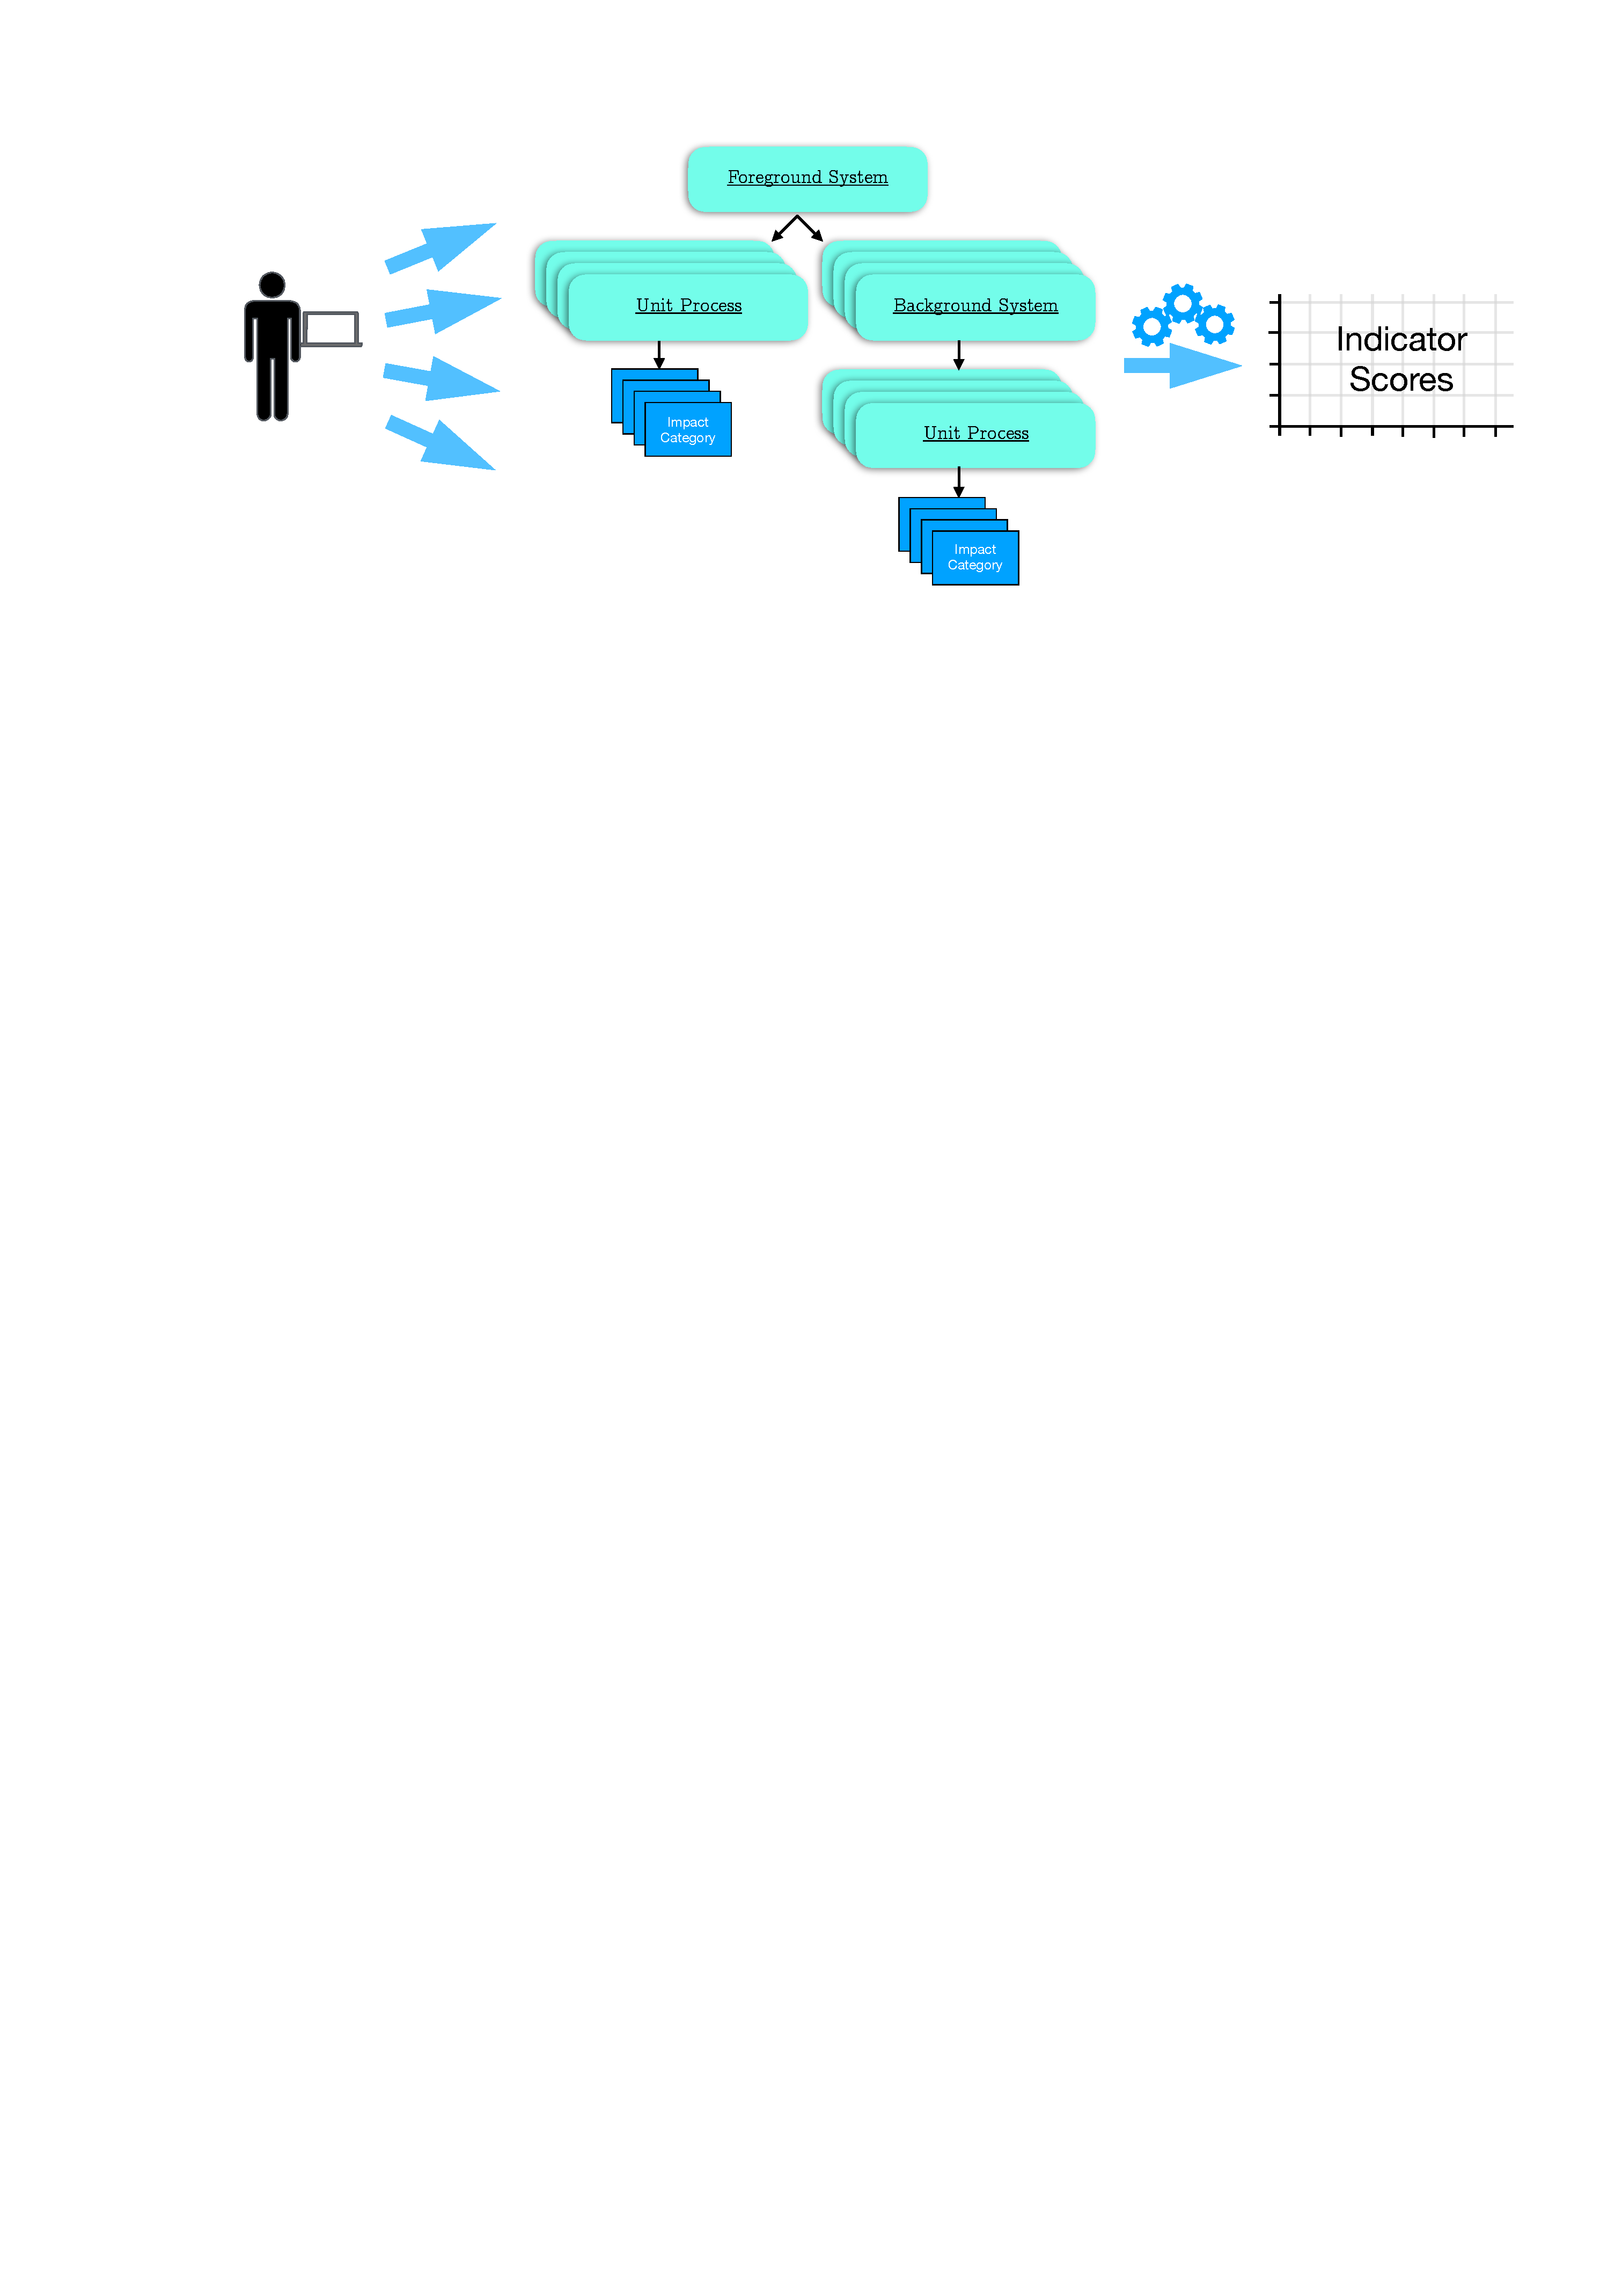
\includegraphics[width = \linewidth]{.figures/ProgramParts.pdf}
\end{figure}
\vfill
\end{frame}

\begin{frame}{Objectives}

\begin{figure}
    \centering
    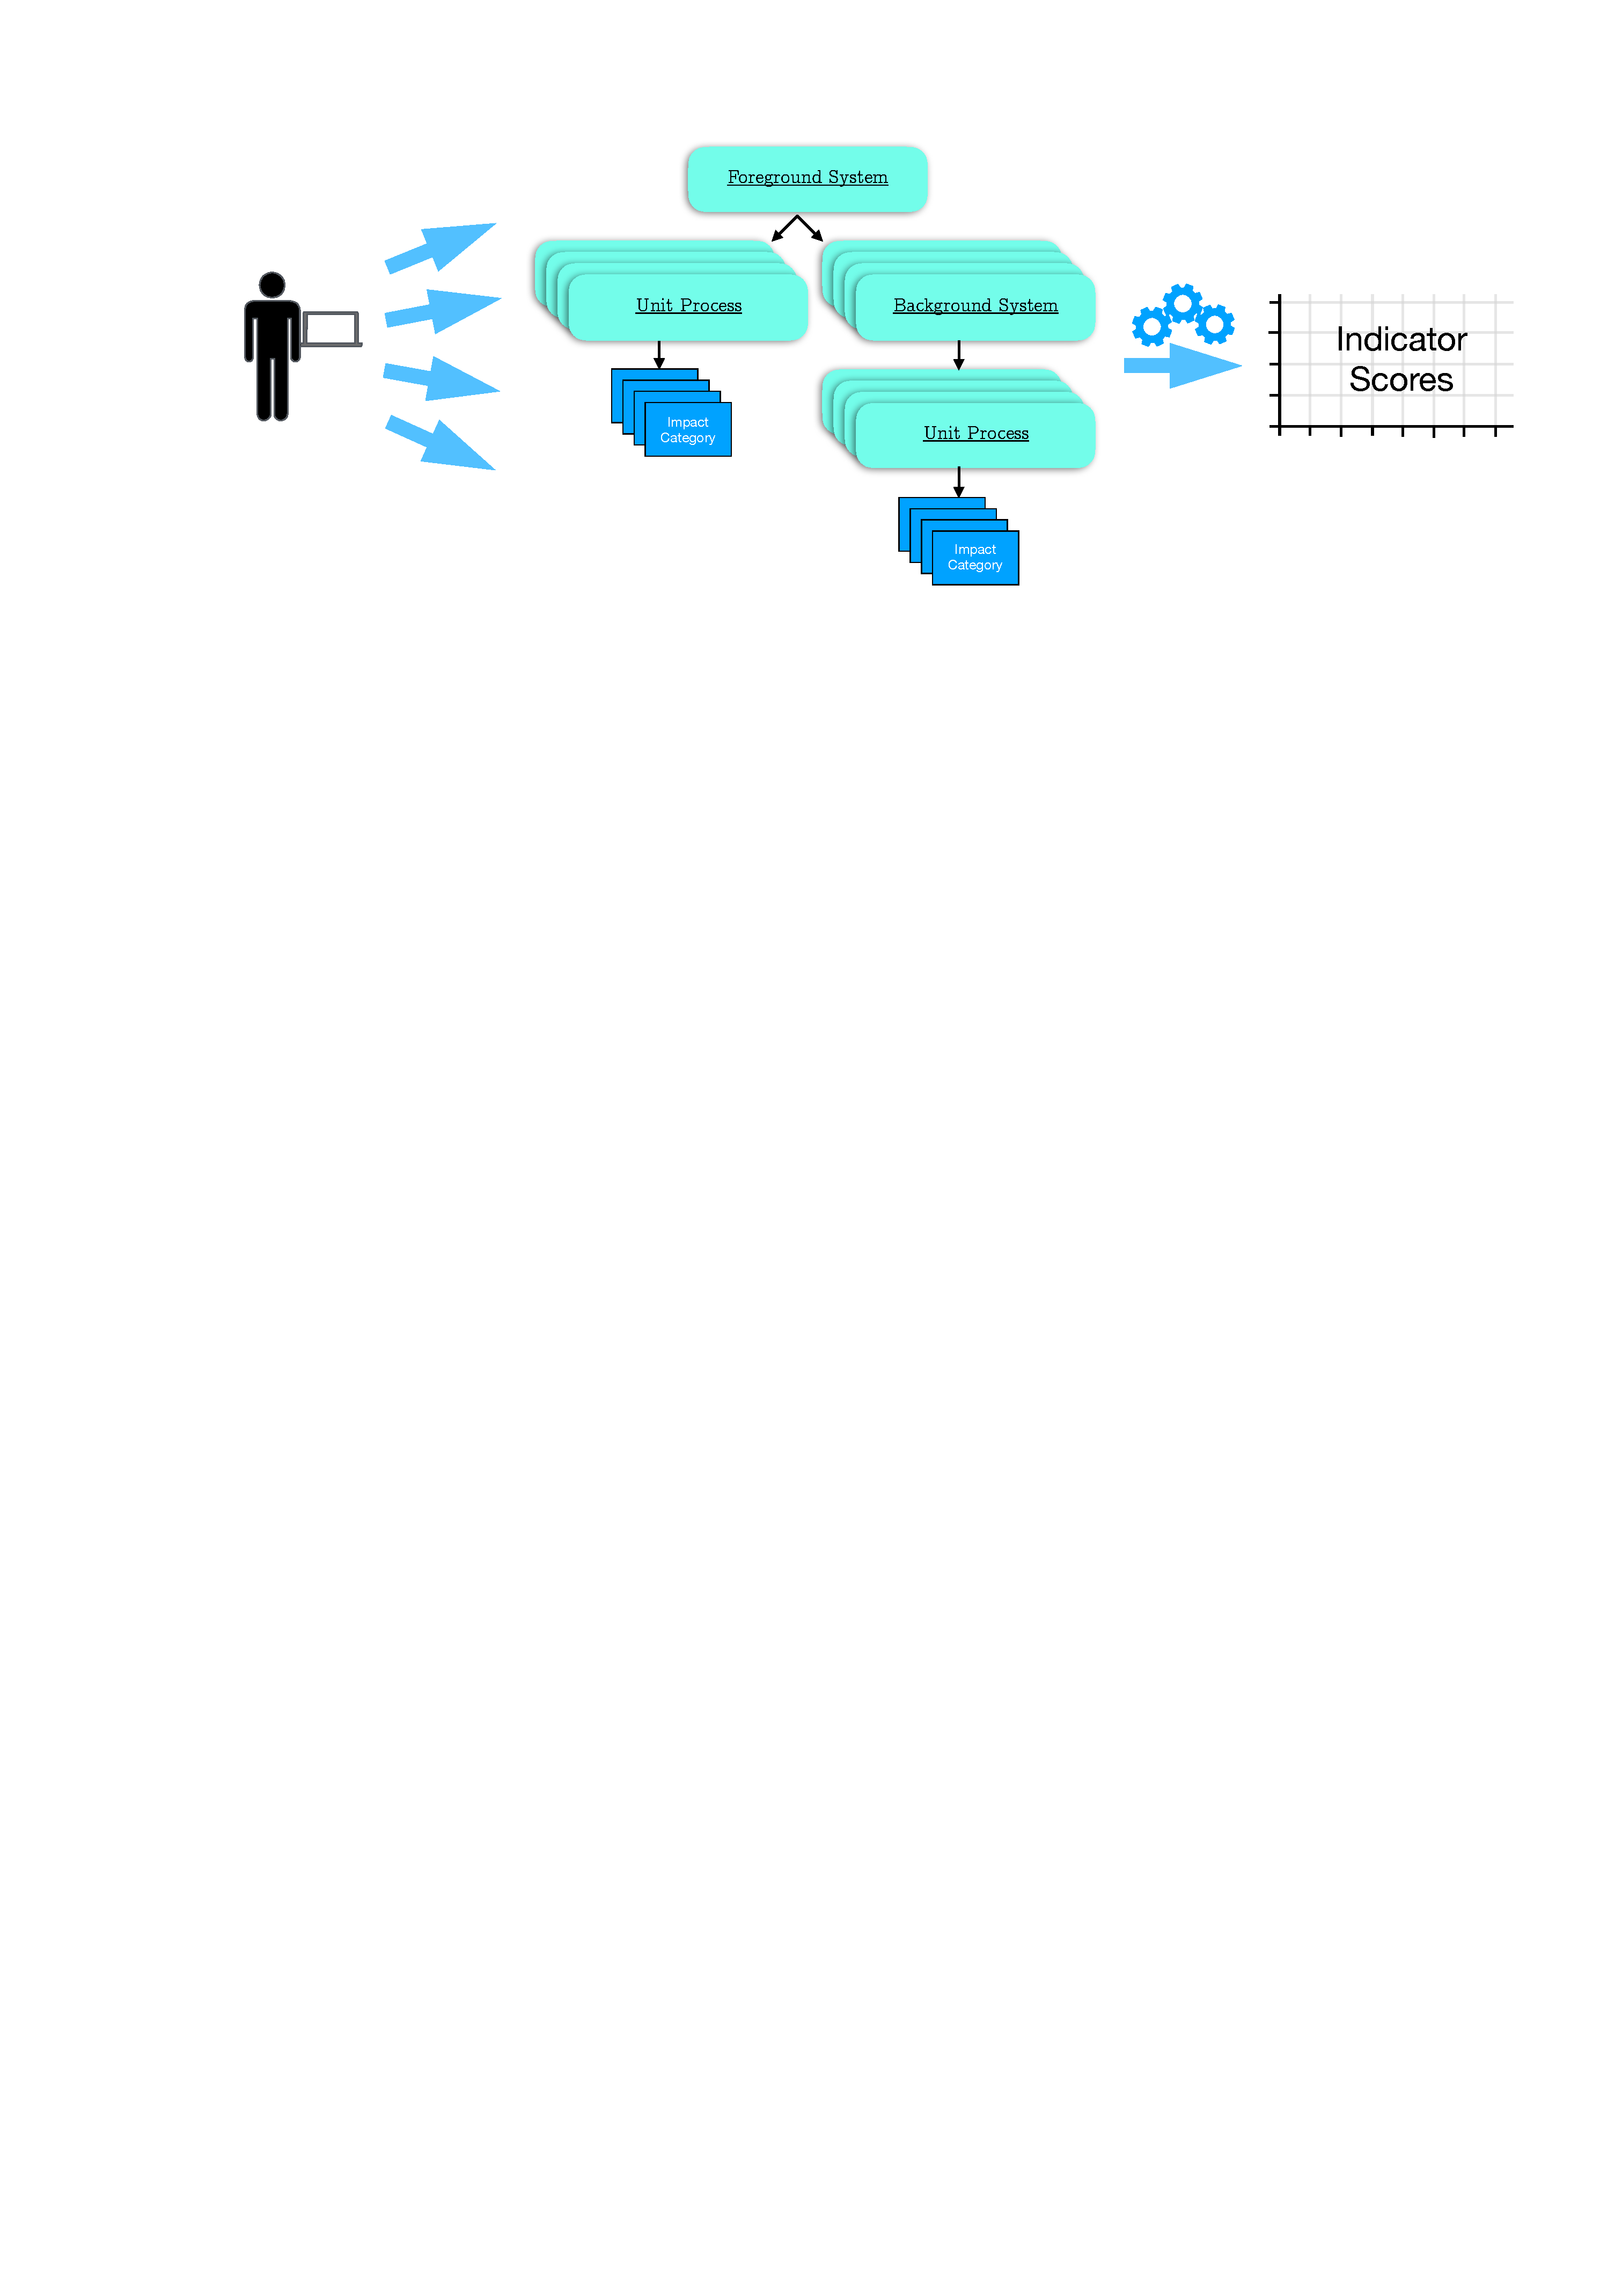
\includegraphics[width = \linewidth]{.figures/ProgramParts.pdf}
\end{figure}

Input $\rightarrow$ Parse $\rightarrow$ LCI model $\rightarrow$ Impact calculation $\rightarrow$ Result

LCI model:\\
LCIA methods, background systems and foreground systems
\vfill
\end{frame}

\begin{frame}{Program Structure}

Design patterns: MVC and IoC

\begin{figure}
    \centering
    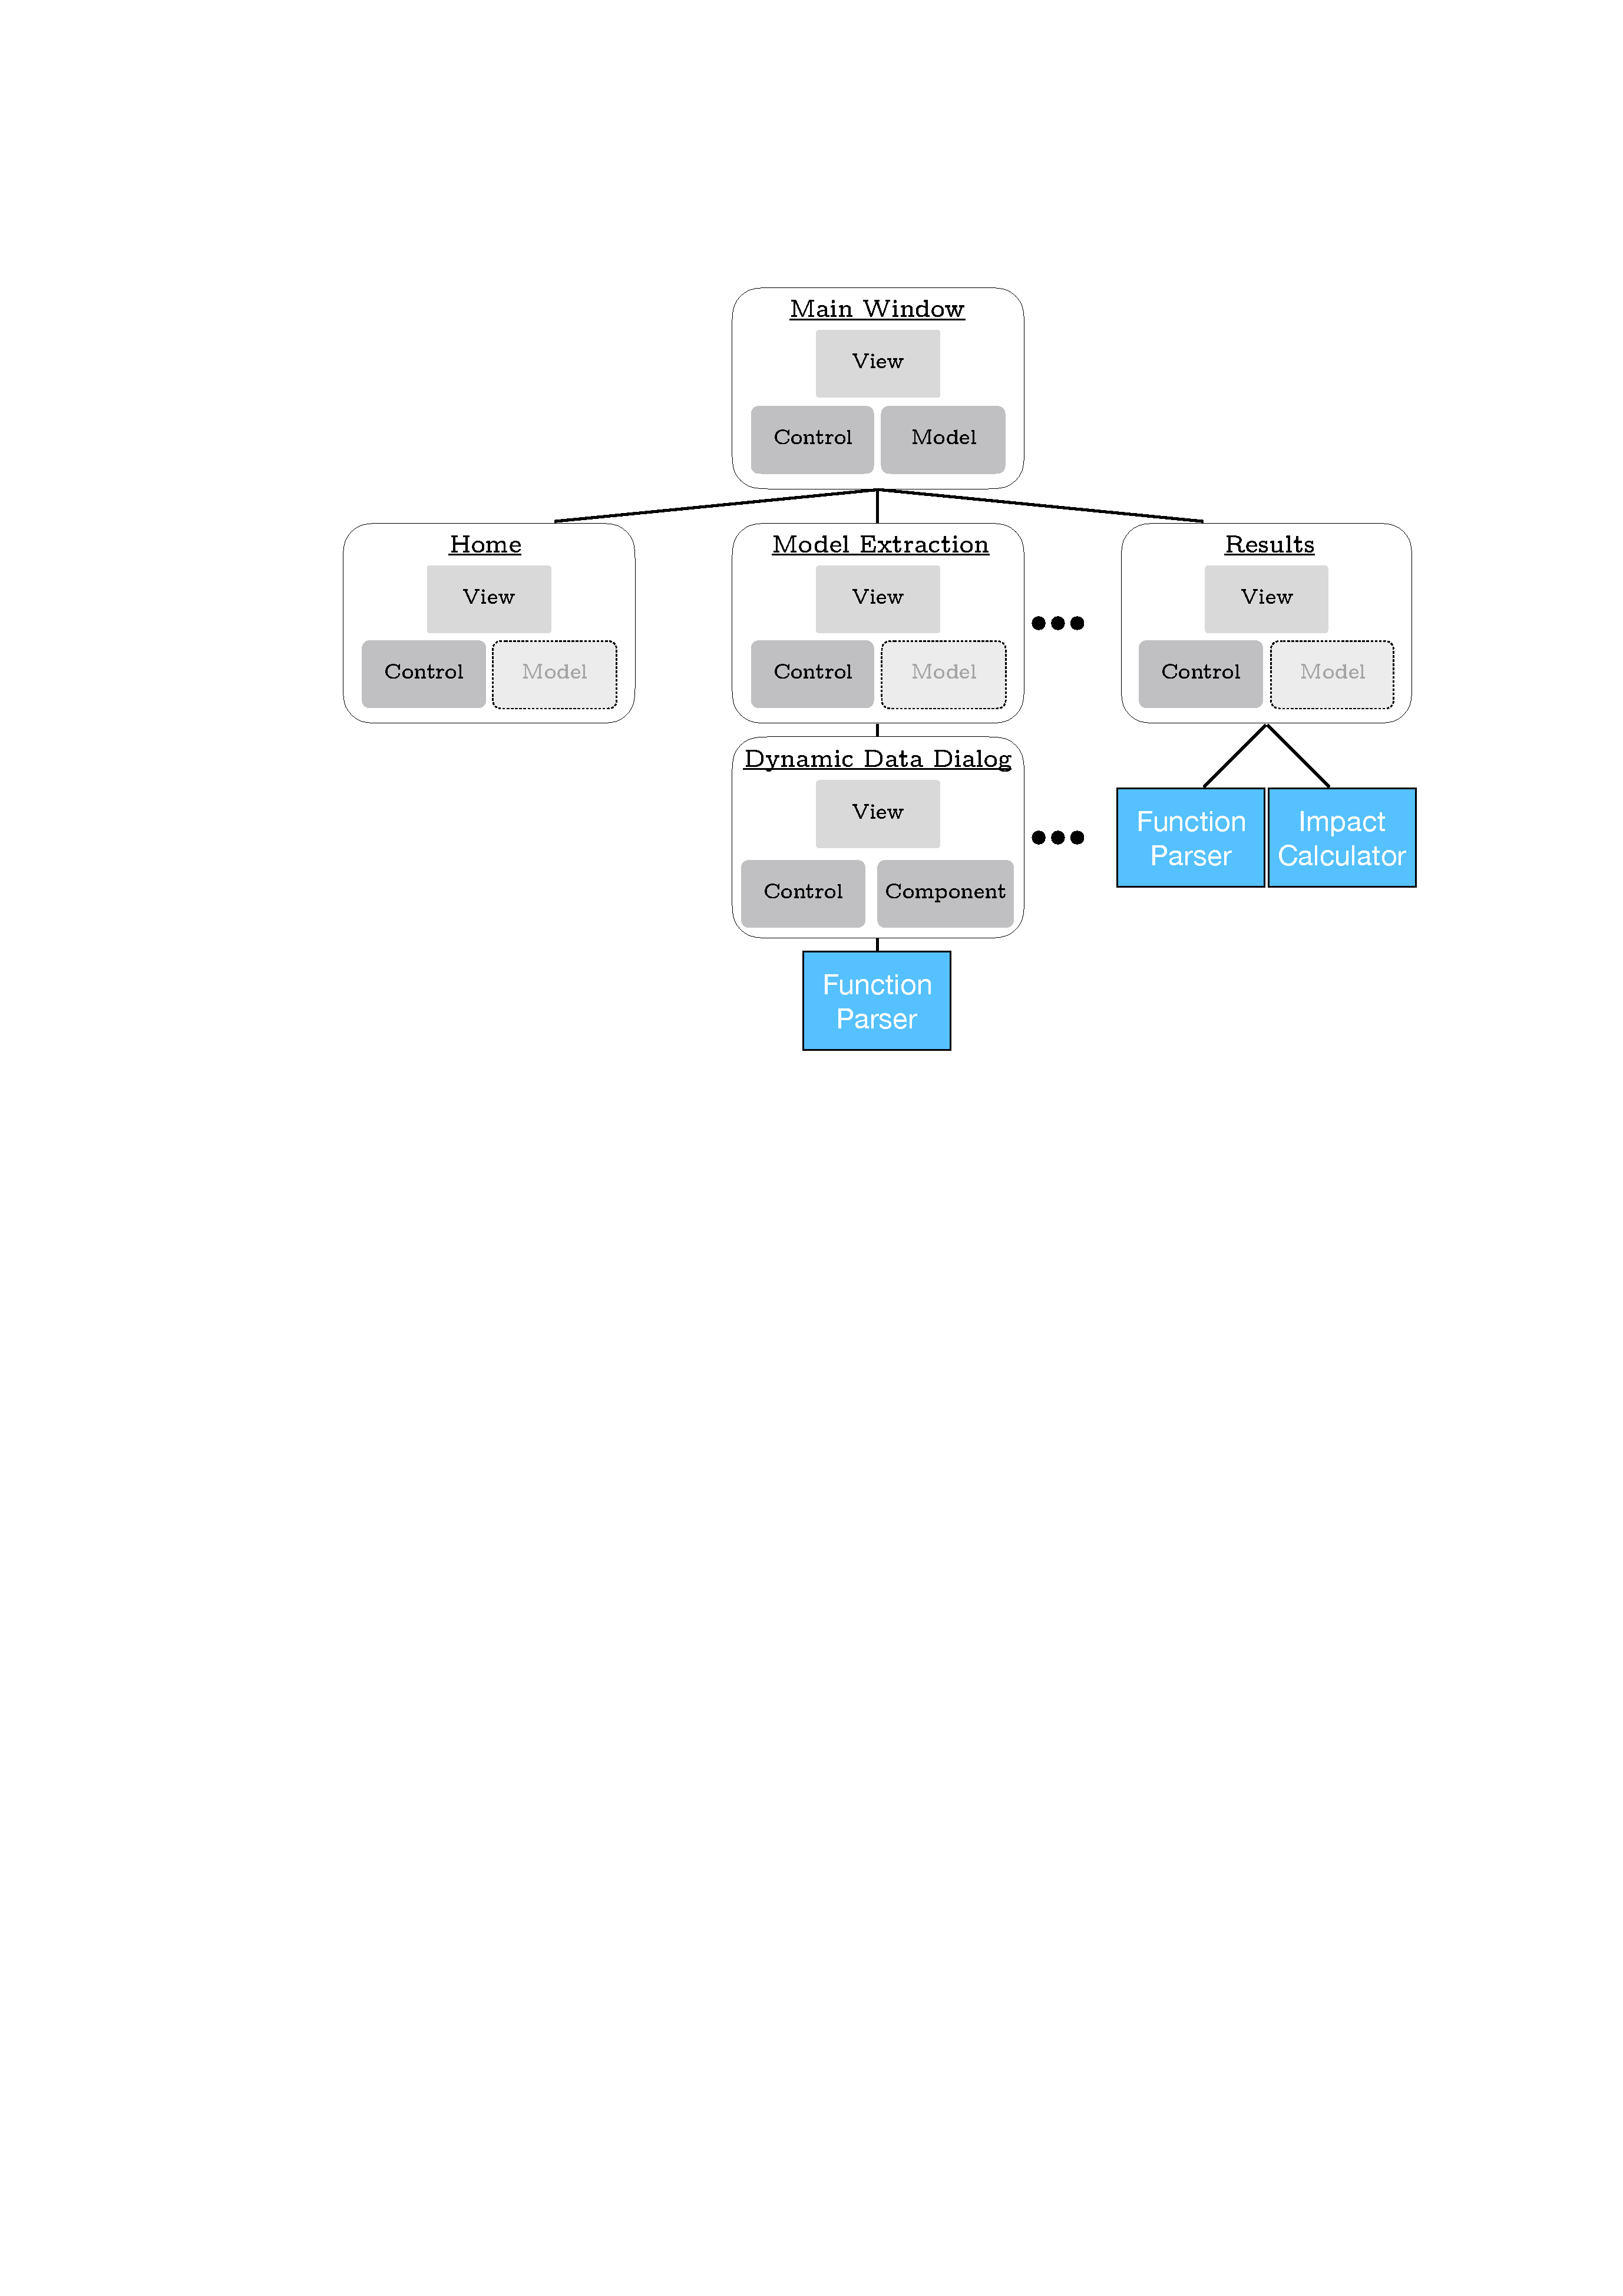
\includegraphics[page=1, width=0.9\linewidth]{.figures/Architecture.pdf}
\end{figure}

\end{frame}
\begin{frame}
\centering
\Large
Testing
\end{frame}
\begin{frame}{Testing}

\emph{Development Testing - Software Engineering ed. 10} \\
\hspace{5mm} by Ian Sommerville.

\vspace{5mm}

\begin{itemize}
    \item Unit Testing
    \item Component Testing
    \item System Testing
\end{itemize}
\end{frame}

\begin{frame}{Unit \& Component Testing}
    \vfill 
    Testing form: Unit tests - White box
    \vfill
    Model units grouped by their components.
    
    \begin{figure}
        \centering
        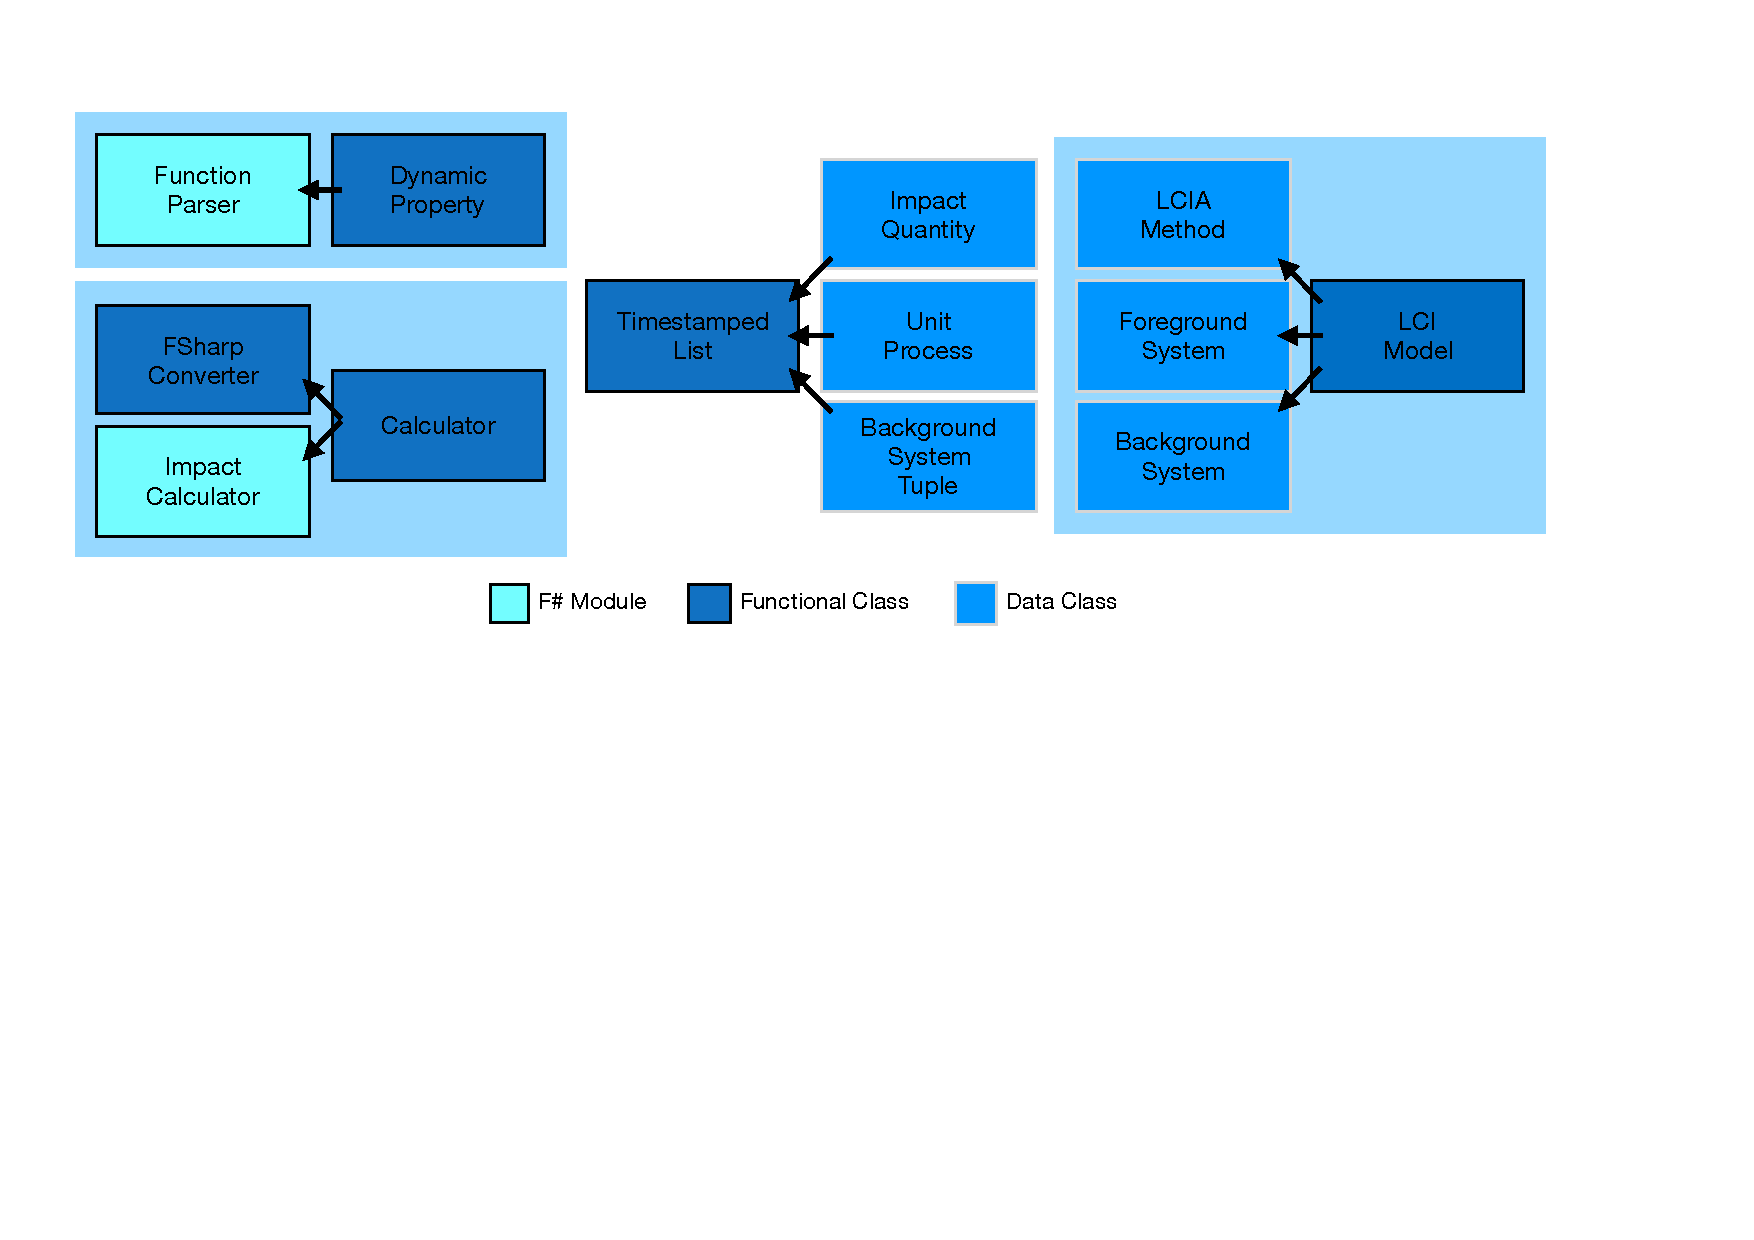
\includegraphics[width=\linewidth]{.figures/TestingGroups.pdf}
    \end{figure}
\end{frame}

\begin{frame}{System Testing}
    Testing form: Scenario tests by use cases - Black box
    \vspace{5mm}
    \begin{figure}
        \centering
        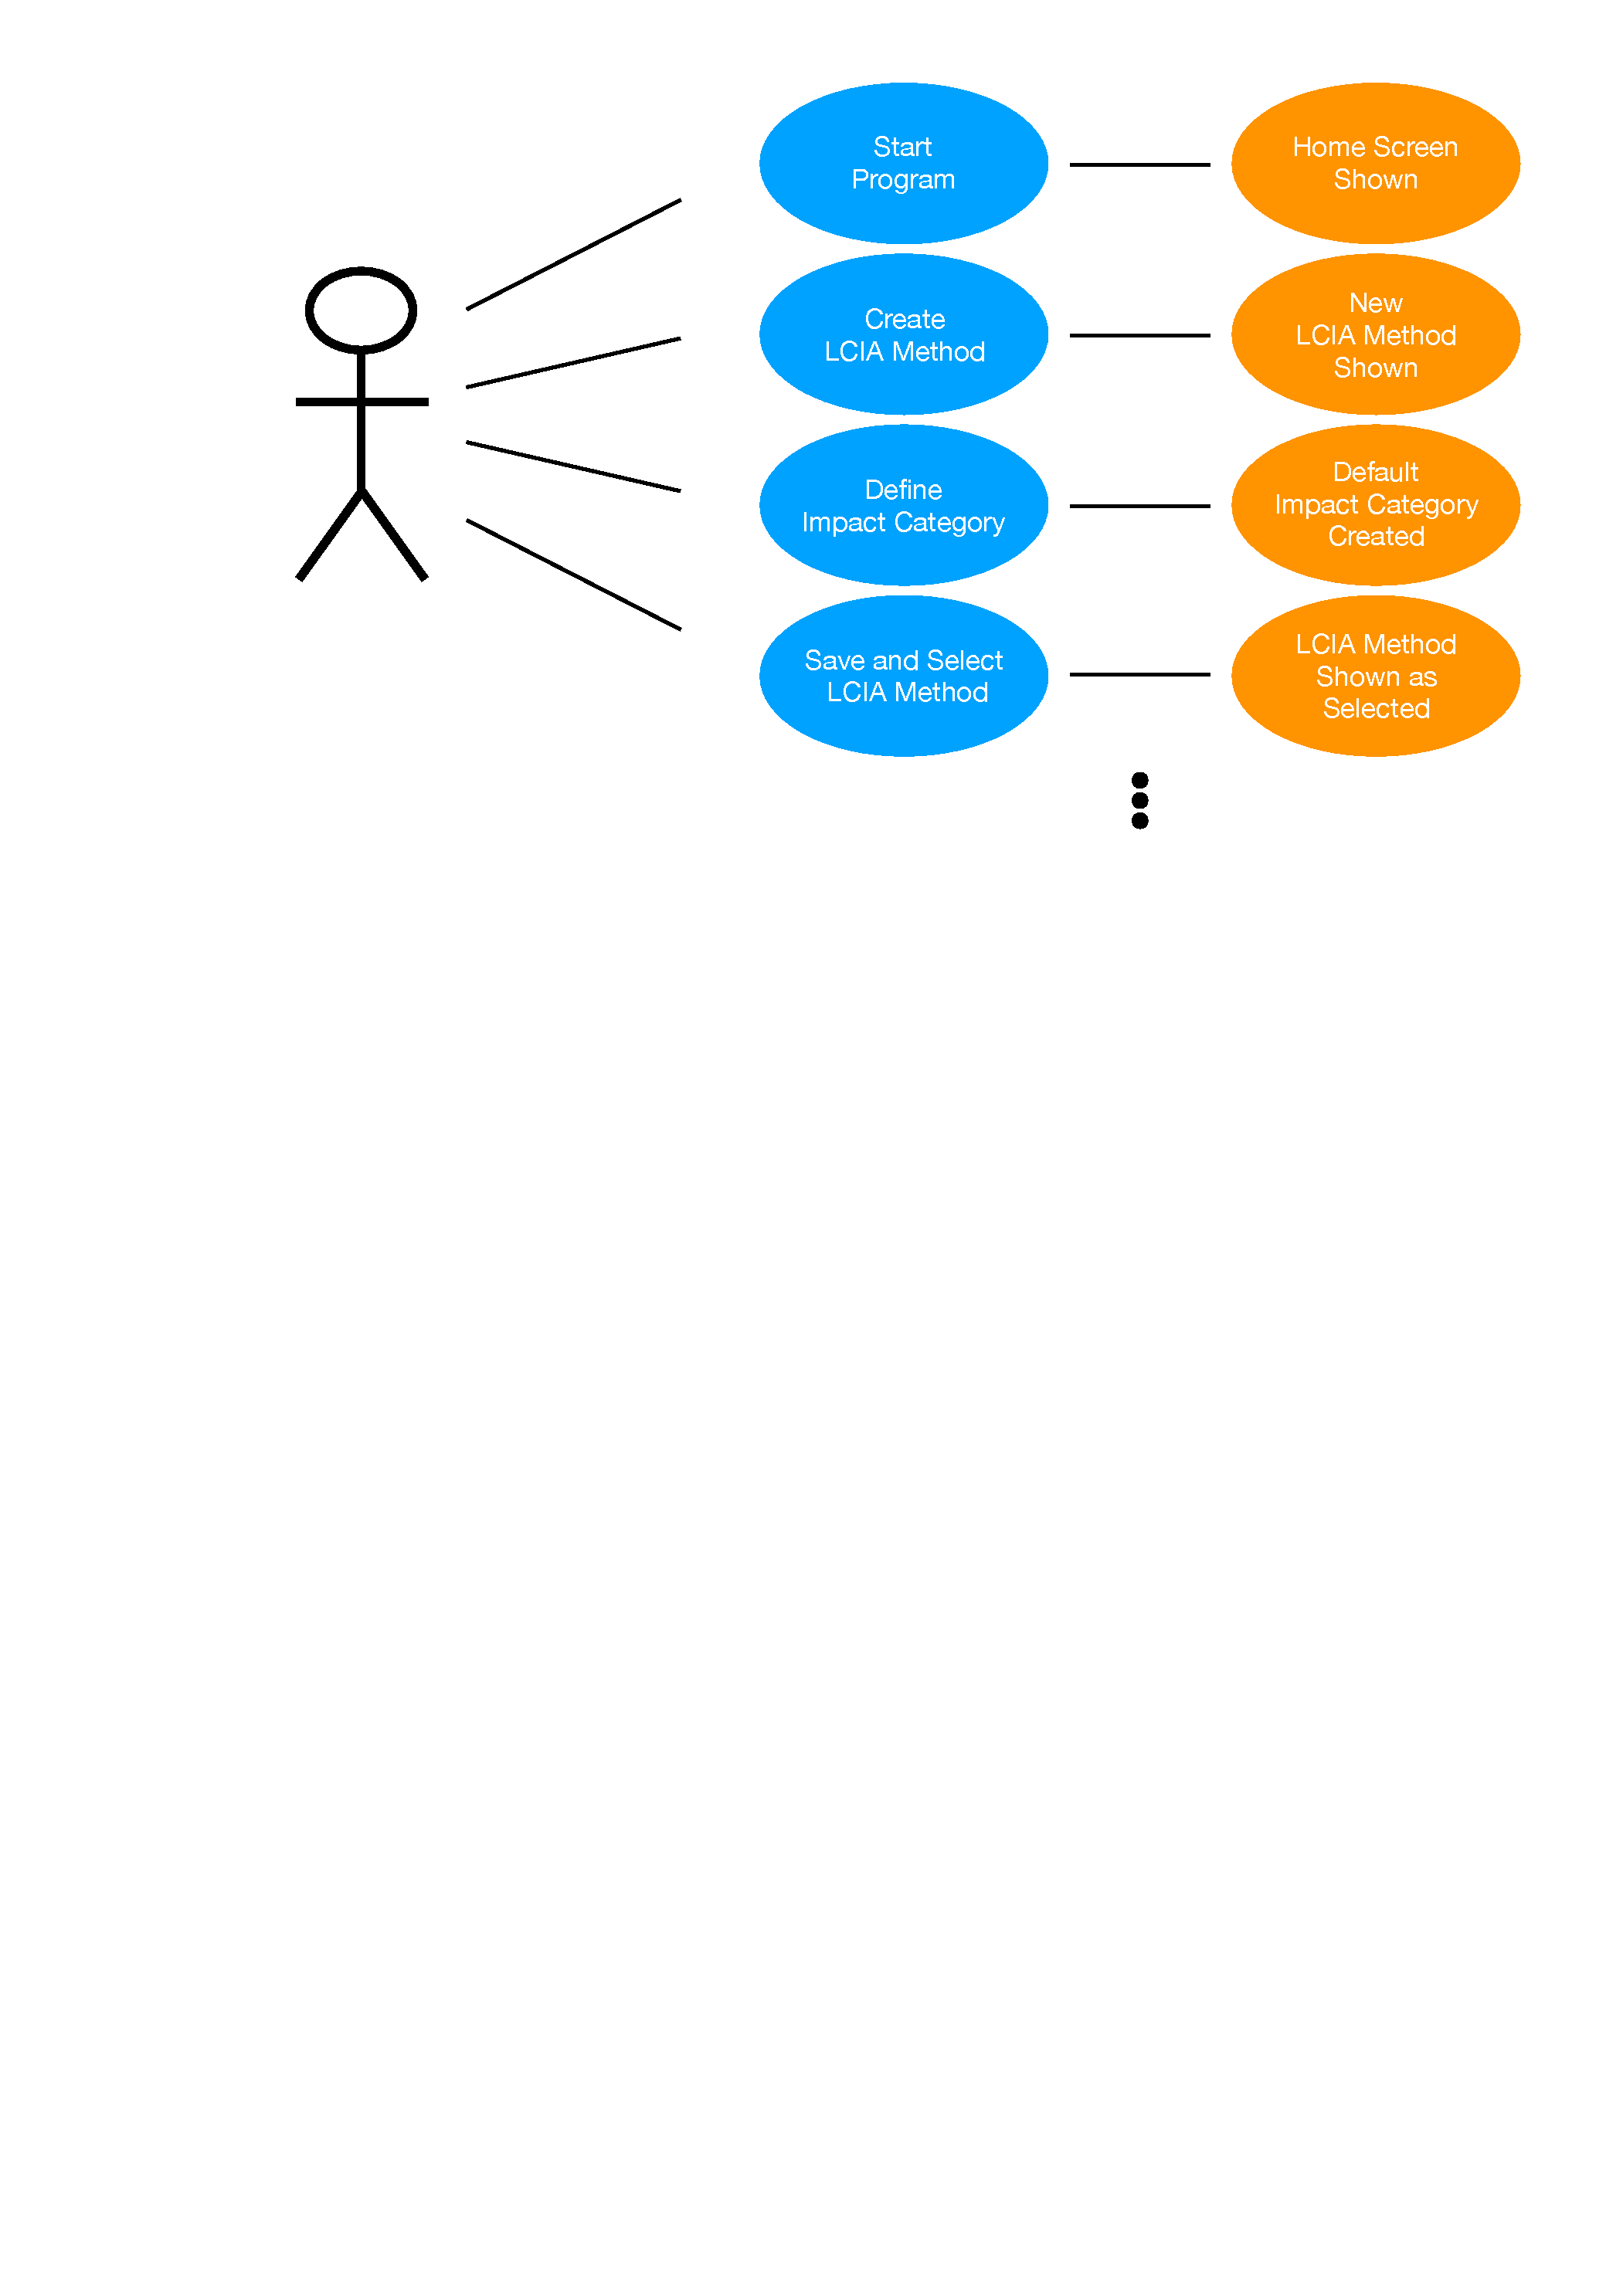
\includegraphics[width=0.7\linewidth]{.figures/ScenarioTesting.pdf}
    \end{figure}
\end{frame}
\begin{frame}
    \centering
    \Large
    Decisions
\end{frame}

\begin{frame}{Function Parsing}
OperatorPrecedenceParser class vs Manual parsing

Grammar - Productions

Semantics - Evaluation function
\end{frame}

\begin{frame}{Function Parsing}
    \begin{figure}
        \centering
        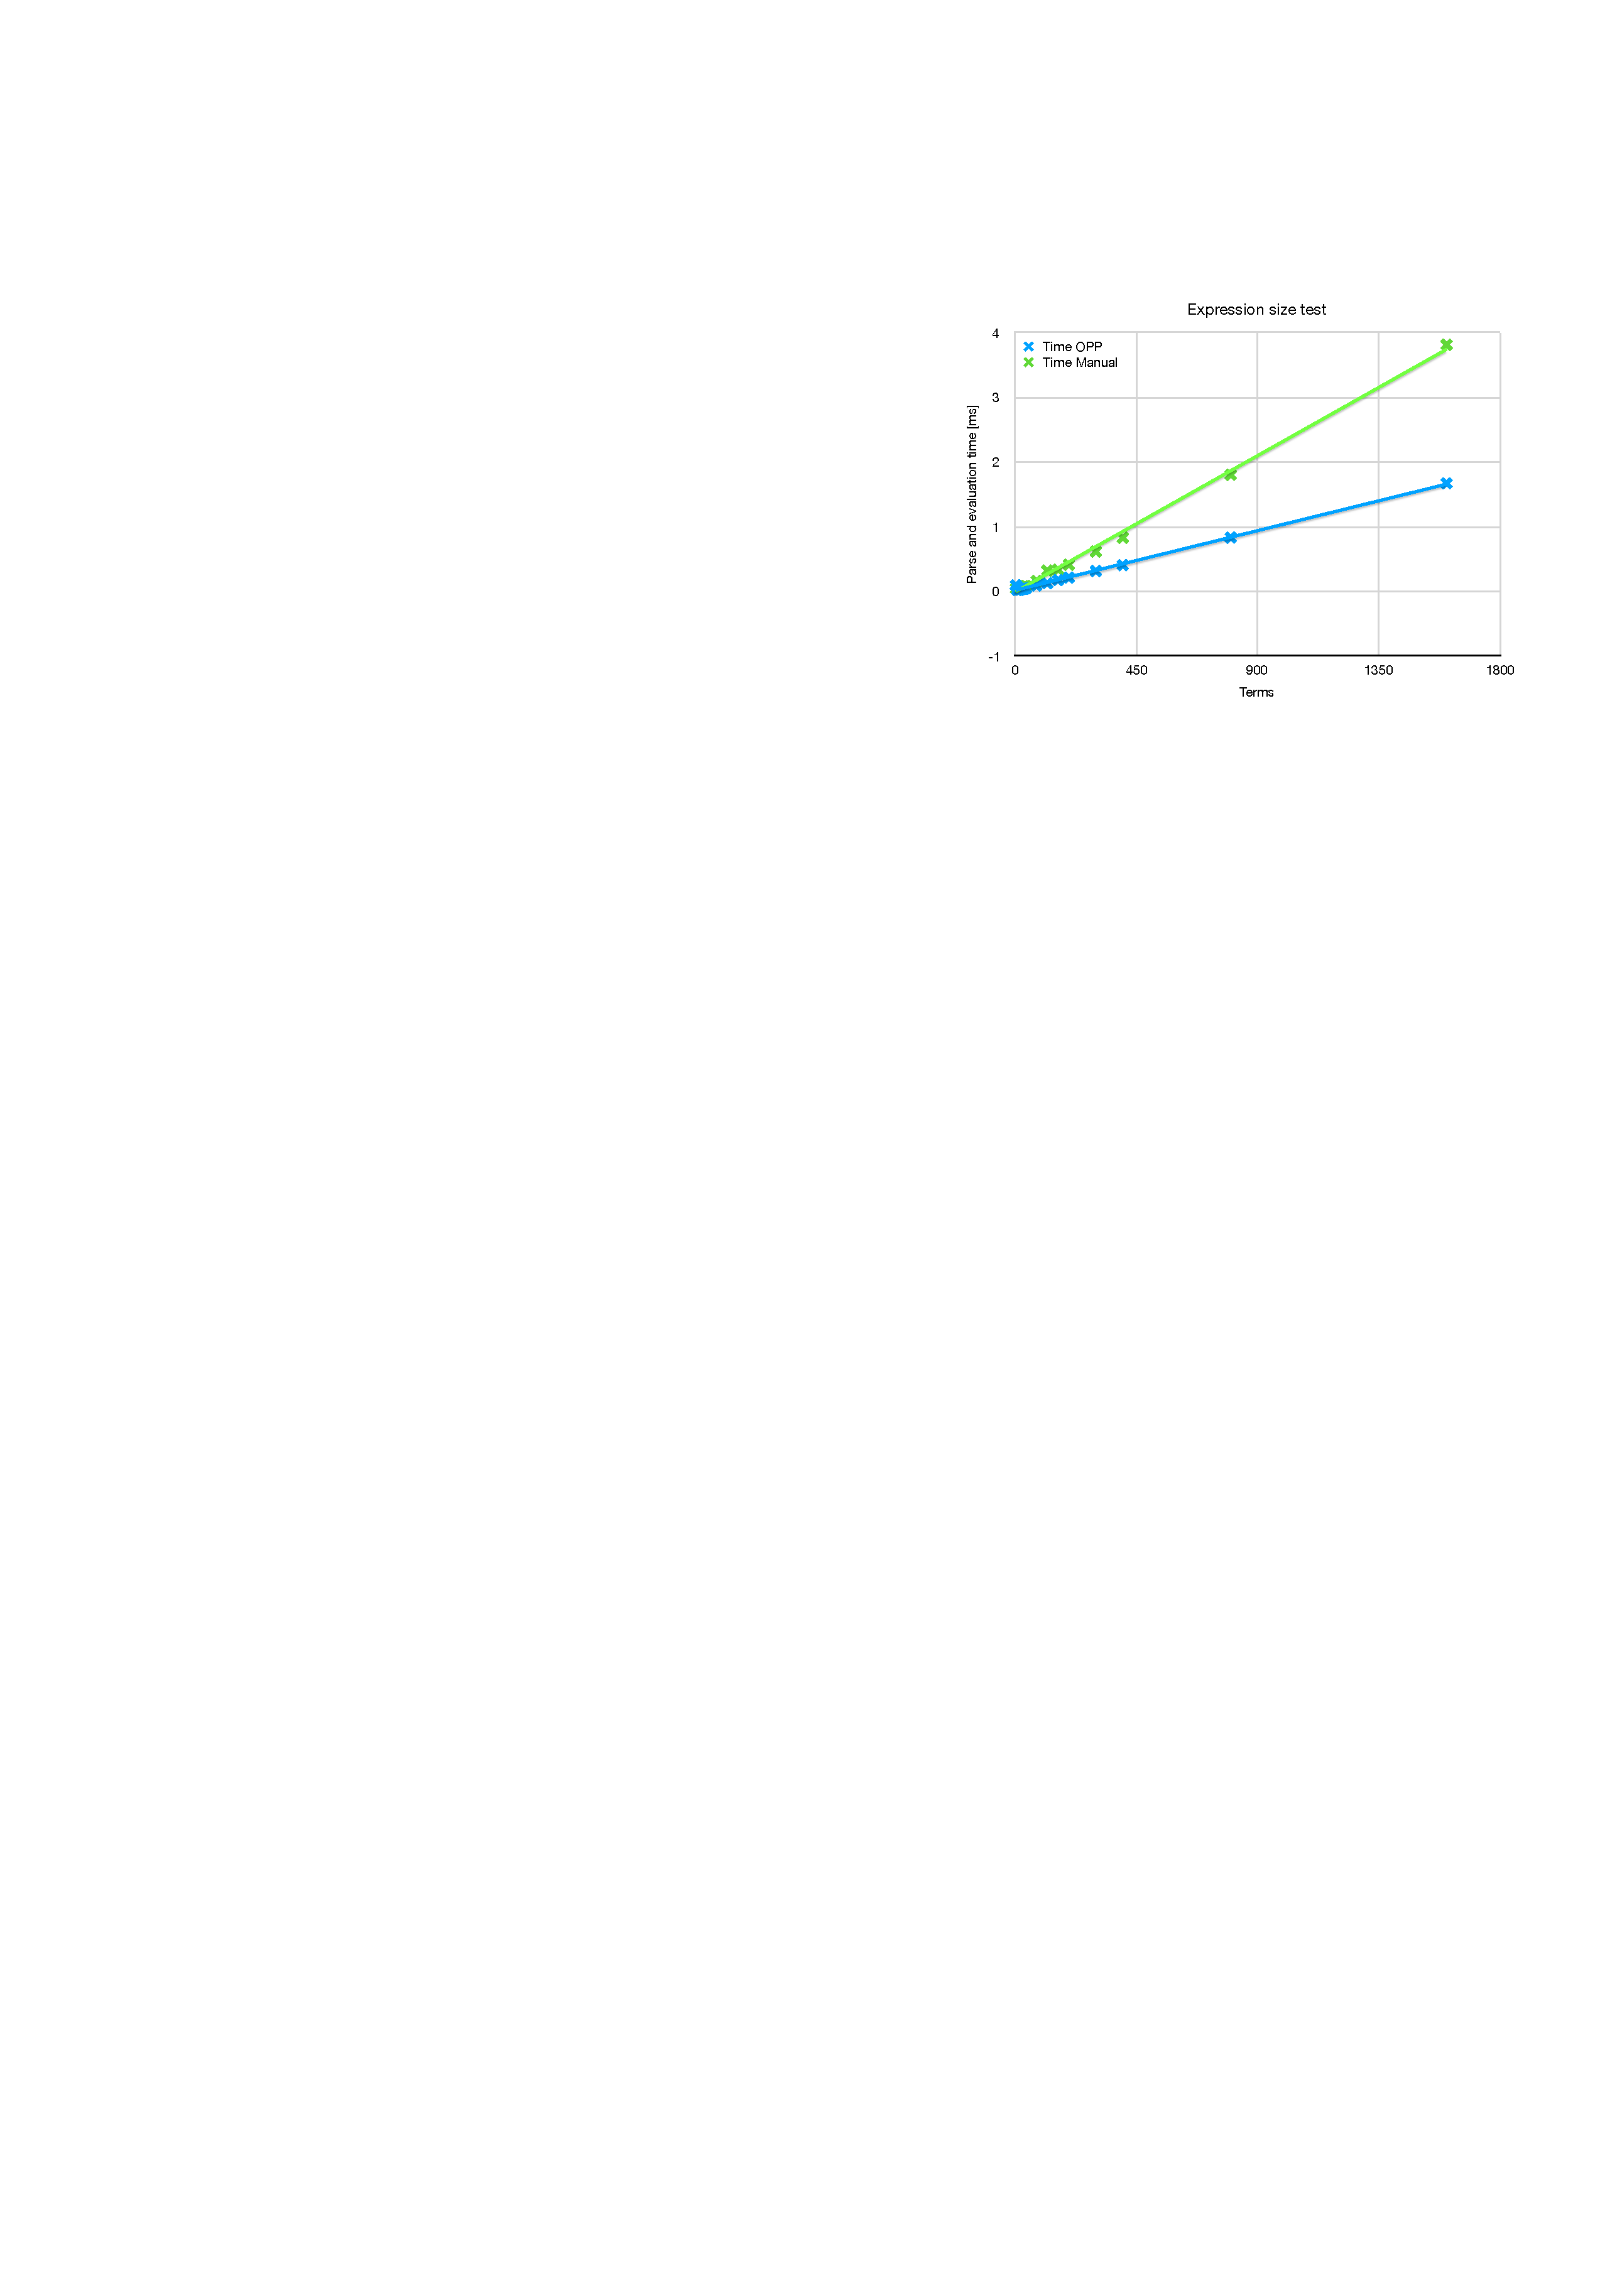
\includegraphics[page=1, width = 0.9\linewidth]{.figures/FunctionParsingTimes.pdf}
    \end{figure}
\end{frame}

\begin{frame}{Function Parsing}
    \begin{figure}
        \centering
        \includegraphics[page=2, width = 0.9\linewidth]{.figures/FunctionParsingTimes.pdf}
    \end{figure}
\end{frame}

\begin{frame}{Impact Calculator}
Calculating individual time steps

Calculating all time steps
\end{frame}

\begin{frame}{Impact Calculator}
\begin{figure}
    \centering
    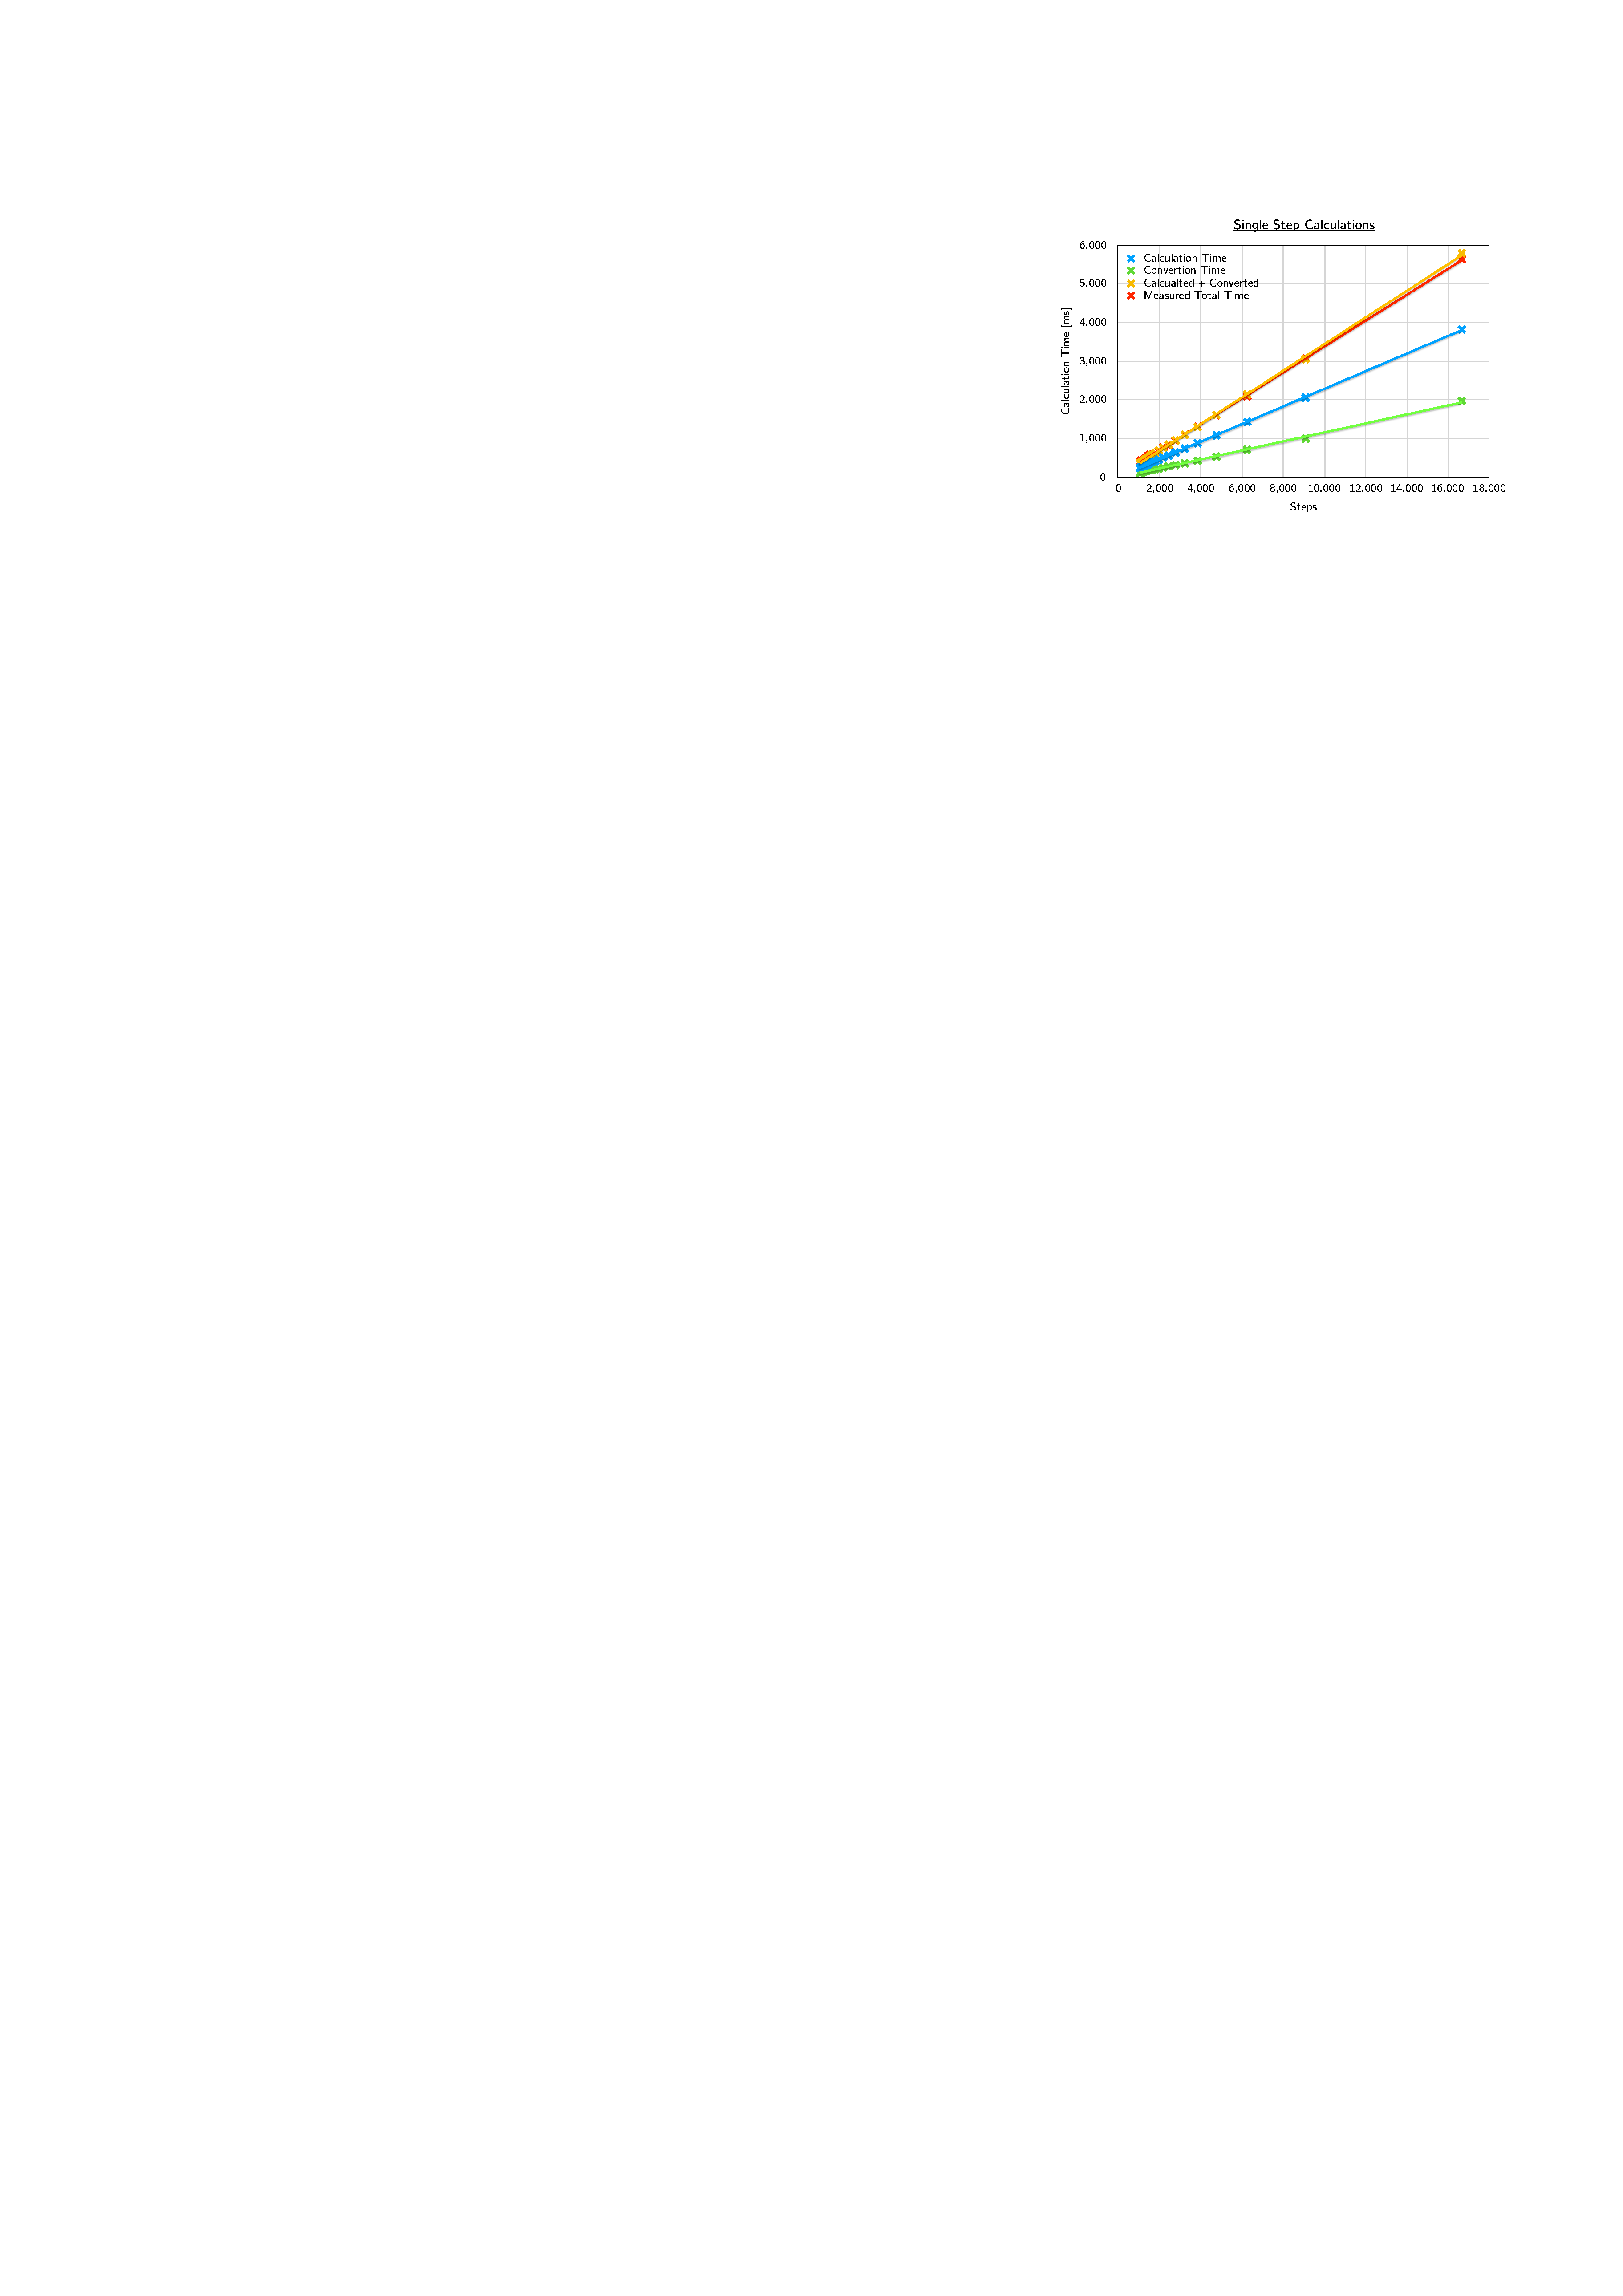
\includegraphics[page=1, width=0.9\linewidth]{.figures/CalculationTimes.pdf}
\end{figure}
\end{frame}

\begin{frame}{Impact Calculator}
\begin{figure}
    \centering
    \includegraphics[page=2, width=0.9\linewidth]{.figures/CalculationTimes.pdf}
\end{figure}
\end{frame}

\begin{frame}{Impact Calculator}
\begin{figure}
    \centering
    \includegraphics[page=3, width=0.9\linewidth]{.figures/CalculationTimes.pdf}
\end{figure}
\end{frame}


\begin{frame}{}
    \centering
    \Huge
    Demo
\end{frame}

\begin{frame}{}
Additional Topics:
\begin{itemize}
    \item Data interpolation (between known data values)
    \item Data extrapolation (after known interval)
    \item Piece-wise functions (dynamic properties)
    \item Event handling (pipelines)
    \item Concurrency (worker thread)
    \item Tools
    \item Use of programming languages
    \item Workflow / Management
    \item Version control
\end{itemize}
\end{frame}

\end{document}